%%%%%%%%%%%%%%%%%%%%%%%% editor.tex %%%%%%%%%%%%%%%%%%%%%%%%%%%%%
%
% sample root file for the contributions of a "contributed volume"
%
% Use this file as a template for your own input.
%
%%%%%%%%%%%%%%%%%%%%%%%%%%%%% Springer %%%%%%%%%%%%%%%%%%%%%%%%%%


% RECOMMENDED %%%%%%%%%%%%%%%%%%%%%%%%%%%%%%%%%%%%%%%%%%%%%%%%%%%
\documentclass[graybox, envcountchap]{styles/svmult}

% general metadata:
\author{soulmachine@gmail.com}
\title{Machine Learning Cheat Sheet}
\subtitle{Insights, diagrams and equations of machine learning}

% choose options for [] as required from the list
% in the Reference Guide

\usepackage{amssymb,amsmath,bm}
\DeclareMathAlphabet{\mathcal}{OMS}{cmsy}{m}{n}
\usepackage{textcomp}
\newcommand\abs[1]{\left\lvert#1\right\rvert}
\usepackage{longtable}
\usepackage{algorithm2e}
\usepackage{tocbibind}
\renewcommand{\bibname}{References}
\usepackage{mathptmx}        % selects Times Roman as basic font
\usepackage{helvet}          % selects Helvetica as sans-serif font
\usepackage{courier}         % selects Courier as typewriter font
%\usepackage{type1cm}        % activate if the above 3 fonts are 
                             % not available on your system

\usepackage{makeidx}         % allows index generation
\usepackage{graphicx}        % standard LaTeX graphics tool
                             % when including figure files
\usepackage[justification=centering]{caption}
\usepackage{multicol}        % used for the two-column index
\usepackage[bottom]{footmisc}% places footnotes at page bottom
\usepackage[bookmarksnumbered=true,
            bookmarksopen=true,
            colorlinks=true,
            linkcolor=blue,
            anchorcolor=blue,
            citecolor=blue
           ]{hyperref}

\graphicspath{{figures/}}

% see the list of further useful packages in the Reference Guide

\makeindex             % used for the subject index
                       % please use the style svind.ist with
                       % your makeindex program

%%%%%%%%%%%%%%%%%%%%%%%%%%%%%%%%%%%%%%%%%%%%%%%%%%%%%%%%%%%%%%%%%

\begin{document}

\frontmatter%%%%%%%%%%%%%%%%%%%%%%%%%%%%%%%%%%%%%%%%%%%%%%%%%%%%%%

\begin{titlepage}

\url{https://github.com/soulmachine/machine-learning-cheat-sheet}

\end{titlepage}

\newpage

\noindent \textcopyright  2013 soulmachine \\
Except where otherwise noted, This document is licensed under a Creative Commons 
Attribution-ShareAlike 3.0 Unported (CC BY-SA3.0) license \\ (\url{http://creativecommons.org/licenses/by/3.0/}).

%%%%%%%%%%%%%%%%%%%%%%%% dedic.tex %%%%%%%%%%%%%%%%%%%%%%%%%%
%
% sample dedication
%
% Use this file as a template for your own input.
%
%%%%%%%%%%%%%%%%%%%%%%%% Springer %%%%%%%%%%%%%%%%%%%%%%%%%%

\begin{dedication}
This book is dedicated to my girl friend Jie Liu, thanks for her companion.
\end{dedication}




%%%%%%%%%%%%%%%%%%%%%%%foreword.tex%%%%%%%%%%%%%%%%%%%%%%%%%%%
% sample foreword
%
% Use this file as a template for your own input.
%
%%%%%%%%%%%%%%%%%%%%%%%% Springer %%%%%%%%%%%%%%%%%%%%%%%%%%

\foreword

Use the template \textit{foreword.tex} together with the Springer document class SVMono (monograph-type books) or SVMult (edited books) to style your foreword\index{foreword} in the Springer layout. 

The foreword covers introductory remarks preceding the text of a book that are written by a \textit{person other than the author or editor} of the book. If applicable, the foreword precedes the preface which is written by the author or editor of the book.


\vspace{\baselineskip}
\begin{flushright}\noindent
Place, month year\hfill {\it Firstname  Surname}\\
\end{flushright}



%%%%%%%%%%%%%%%%%%%%%%preface.tex%%%%%%%%%%%%%%%%%%%%%%%%%%%%%%%%%%%%%%%%%
% sample preface
%
% Use this file as a template for your own input.
%
%%%%%%%%%%%%%%%%%%%%%%%% Springer %%%%%%%%%%%%%%%%%%%%%%%%%%

\preface

This cheat sheet contains many classical equations and diagrams on machine learning, which will help you quickly recall knowledge and ideas in machine learning.

This cheat sheet has three significant advantages:
\begin{enumerate}
\item Strong typed. Compared to programming languages, mathematical formulas are weekly typed. For example, $X$ can be a set, a random variable, or a matrix. This causes difficulty in understanding the meaning of formulas. In this cheat sheet, I try my best to standardize symbols used, see section \S \ref{sec:Notation}.
\item More parentheses. In machine leaning, authors are prone to omit parentheses, brackets and braces,  this usually causes ambiguity in mathematical formulas. In this cheat sheet, I use parentheses(brackets and braces) at where they are needed, to make formulas easy to understand.
\item Less thinking jumps. In many books, authors are prone to omit some steps that are trivial in his option. But it often makes readers get lost in the middle way of derivation.
\end{enumerate}

\vspace{\baselineskip}
\begin{flushright}\noindent
At Tsinghua University, May 2013\hfill {\it soulmachine} \\
\end{flushright}



%%%%%%%%%%%%%%%%%%%%%%%acknow.tex%%%%%%%%%%%%%%%%%%%%%%%%%%%%%%%%%%%%%%%%%
% sample acknowledgement chapter
%
% Use this file as a template for your own input.
%
%%%%%%%%%%%%%%%%%%%%%%%% Springer %%%%%%%%%%%%%%%%%%%%%%%%%%

\extrachap{Acknowledgements}

Use the template \emph{acknow.tex} together with the Springer document class SVMono (monograph-type books) or SVMult (edited books) if you prefer to set your acknowledgement section as a separate chapter instead of including it as last part of your preface.



\tableofcontents
%%%%%%%%%%%%%%%%%%%%clist.tex %%%%%%%%%%%%%%%%%%%%%%%%
%                                                    
% sample list of contributors and their addresses    
%                                                    
% Use this file as a template for your own input.    
%                                                    
%%%%%%%%%%%%%%%%%%%%%%%% Springer %%%%%%%%%%%%%%%%%%%%
\contributors

\begin{thecontriblist}
Wei Zhang
\at PhD candidate at the Institute of Software, Chinese Academy of Sciences (ISCAS), Beijing, P.R.CHINA, \email{zh3feng@gmail.com}, has written chapters of Naive Bayes and SVM.
\and
Fei Pan
\at Master at Beijing University of Technology, Beijing, P.R.CHINA, \email{example@gmail.com}, has written chapters of KMeans, AdaBoost.
\and
Yong Li
\at PhD candidate at the Institute of Automation of the Chinese Academy of Sciences (CASIA), Beijing, P.R.CHINA, \email{liyong3forever@gmail.com}, has written chapters of Logistic Regression.
\and
Jiankou Li
\at PhD candidate at the Institute of Software, Chinese Academy of Sciences (ISCAS), Beijing, P.R.CHINA, \email{lijiankoucoco@163.com}, has written chapters of BayesNet.
\end{thecontriblist}
%%%%%%%%%%%%%%%%%%%%%%%acronym.tex%%%%%%%%%%%%%%%%%%%%%%%%%%%%%%%%%%%%%%%%%
% sample list of acronyms
%
% Use this file as a template for your own input.
%
%%%%%%%%%%%%%%%%%%%%%%%% Springer %%%%%%%%%%%%%%%%%%%%%%%%%%

\extrachap{Acronyms}

Use the template \emph{acronym.tex} together with the Springer document class SVMono (monograph-type books) or SVMult (edited books) to style your list(s) of abbreviations or symbols in the Springer layout.

Lists of abbreviations\index{acronyms, list of}, symbols\index{symbols, list of} and the like are easily formatted with the help of the Springer-enhanced \verb|description| environment.

\begin{description}[CABR]
\item[ABC]{Spelled-out abbreviation and definition}
\item[BABI]{Spelled-out abbreviation and definition}
\item[CABR]{Spelled-out abbreviation and definition}
\end{description}
\Extrachap{Notation}
\label{sec:Notation}

\section*{Introduction}
It is very difficult to come up with a single, consistent notation to cover the wide variety of
data, models and algorithms that we discuss. Furthermore, conventions difer between machine
learning and statistics, and between different books and papers. Nevertheless, we have tried
to be as consistent as possible. Below we summarize most of the notation used in this book,
although individual sections may introduce new notation. Note also that the same symbol may
have different meanings depending on the context, although we try to avoid this where possible.


\section*{General math notation}

\begin{longtable}{ll}
\hline\noalign{\smallskip}
\textbf{Symbol} & \textbf{Meaning} \\
\noalign{\smallskip}\hline\noalign{\smallskip}
$\lfloor x \rfloor$ & Floor of $x$, i.e., round down to nearest integer\\
$\lceil x \rceil$ & Ceiling of $x$, i.e., round down to nearest integer\\
$\vec{x} \otimes \vec{y}$ & Convolution of $\vec{x}$ and $\vec{y}$\\
$\vec{x} \odot \vec{y}$ & Hadamard (elementwise) product of $\vec{x}$ and $\vec{y}$\\
$a \wedge b$ & logical AND\\
$a \vee b$ & logical OR\\
$\neg a$ & logical NOT\\
$\mathbb{I}(x)$ & Indicator function, $\mathbb{I}(x)=1$ if x is true, else $\mathbb{I}(x)=0$\\
$\infty$ & Infinity\\
$\rightarrow$ & Tends towards, e.g., $n \rightarrow \infty$\\
$\propto$ &Proportional to, so $y = ax$ can be written as $y \propto x$\\
$\abs{x}$ & Absolute value\\
$\abs{\mathcal{S}}$ & Size (cardinality) of a set\\
$n!$ & Factorial function\\
$\nabla$ & Vector of first derivatives\\
$\nabla^2$ & Hessian matrix of second derivatives\\
$\triangleq$ & Defined as\\
$O(\cdot)$ & Big-O: roughly means order of magnitude\\
$\mathbb{R}$ & The real numbers\\
$1:n$ & Range (Matlab convention): $1:n = {1, 2,...,n}$\\
$\approx$ & Approximately equal to\\
$\arg\max\limits_x f(x)$ & Argmax: the value $x$ that maximizes $f$\\
$B(a,b)$ & Beta function, $B(a,b)=\dfrac{\Gamma(a)\Gamma(b)}{\Gamma(a+b)}$\\
$B(\vec{\alpha})$ & Multivariate beta function, $\dfrac{\prod\limits_k \Gamma(\alpha_k)}{\Gamma(\sum\limits_k \alpha_k)}$\\
$\binom{n}{k}$ & $n$ choose $k$ , equal to $n!/(k!(n−k )!)$\\
$\delta(x)$ & Dirac delta function,$\delta(x)=\infty$ if $x=0$, else $\delta(x)=0$\\
$exp(x)$ & Exponential function $e^x$\\
$\Gamma(x)$ & Gamma function, $\Gamma(x)=\int_0^\infty u^{x-1}e^{-u}\mathrm{d}u$\\
$\Psi(x)$ &  Digamma function,$Psi(x)=\dfrac{d}{dx}\log\Gamma(x)$\\
$\mathcal{X}$ & A set from which values are drawn (e.g.,$\mathcal{X}=\mathbb{R}^D$)\\
\noalign{\smallskip}\hline\noalign{\smallskip}
\end{longtable}


\section*{Linear algebra notation}
We use boldface lower-case to denote vectors, such as $\vec{x}$, and boldface upper-case to denote matrices, such as $\vec{X}$. We denote entries in a matrix by non-bold upper case letters, such as $X_{ij}$. 

Vectors are assumed to be column vectors, unless noted otherwise. We use $(x_1,\cdots,x_D)$ to denote a column vector created by stacking $D$ scalars. If we write $\vec{X}=(\vec{x}_1,\cdots,\vec{x}_n)$, where the left hand side is a matrix, we mean to stack the $\vec{x}_i$ along the columns, creating a matrix. 

\begin{longtable}{ll}
\hline\noalign{\smallskip}
\textbf{Symbol} & \textbf{Meaning} \\
\noalign{\smallskip}\hline\noalign{\smallskip}
$\vec{X} \succ 0$ & $\vec{X}$ is a positive definite matrix\\
$tr(\vec{X})$ & Trace of a matrix\\
$det(\vec{X})$ & Determinant of matrix $\vec{X}$\\
$\abs{\vec{X}}$ & Determinant of matrix $\vec{X}$\\
$\vec{X}^{-1}$ & Inverse of a matrix\\
$\vec{X}^{\dagger}$ & Pseudo-inverse of a matrix\\
$\vec{X}^T$ & Transpose of a matrix\\
$\vec{x}^T$ & Transpose of a vector\\
$diag(x)$ & Diagonal matrix made from vector $\vec{x}$\\
$diag(X)$ & Diagonal vector extracted from matrix $\vec{X}$\\
$\vec{I}$ or $\vec{I}_d$ & Identity matrix of size $d \times d$ (ones on diagonal, zeros of)\\
$\vec{1}$ or $\vec{1}_d$ & Vector of ones (of length $d$)\\
$\vec{0}$ or $\vec{0}_d$ & Vector of zeros (of length $d$)\\
$\abs{\abs{\vec{x}}}=\abs{\abs{\vec{x}}}_2$ & Euclidean or $\ell_2$ norm $\sqrt{\sum\limits_{j=1}^{d} x_j^2}$\\
$\abs{\abs{\vec{x}}}_1$ & $\ell_1$ norm $\sum\limits_{j=1}^{d} \abs{x_j}$\\
$\vec{X}_{:,j}$ & j'th column of matrix\\
$\vec{X}_{i,:}$ & transpose of $i$'th row of matrix (a column vector)\\
$\vec{X}_{i,j}$ & Element $(i,j)$ of matrix $\vec{X}$ \\
$\vec{x} \otimes \vec{y}$ & Tensor product of $\vec{x}$ and $\vec{y}$\\
\noalign{\smallskip}\hline\noalign{\smallskip}
\end{longtable}


\section*{Probability notation}
We denote random and fixed scalars by lower case, random and fixed vectors by bold lower case, and random and fixed matrices by bold upper case. Occasionally we use non-bold upper case to denote scalar random variables. Also, we use $p()$ for both discrete and continuous random variables

\begin{longtable}{ll}
\hline\noalign{\smallskip}
\textbf{Symbol} & \textbf{Meaning} \\
\noalign{\smallskip}\hline\noalign{\smallskip}
$X,Y$ & Random variable\\
$P()$ & Probability of a random event\\
$F()$ & Cumulative distribution function(CDF), also called distribution function\\
$p(x)$ & Probability mass function(PMF)\\
$f(x)$ & probability density function(PDF) \\
$F(x,y)$ & Joint CDF\\
$p(x,y)$ & Joint PMF \\
$f(x,y)$ & Joint PDF\\
$p(X|Y)$ & Conditional PMF, also called conditional probability\\
$f_{X|Y}(x|y)$ & Conditional PDF\\
$X \perp Y$ & X is independent of Y\\
$X \not\perp Y$ & X is not independent of Y\\
$X \perp Y | Z $ & X is conditionally independent of Y given Z\\
$X \not\perp Y | Z $ & X is not conditionally independent of Y given Z\\
$X \sim p$ & X is distributed according to distribution $p$\\
$\vec{\alpha}$ & Parameters of a Beta or Dirichlet distribution\\
$\mathrn{cov}[X]$ & Covariance of X\\
$\mathbb{E}[X]$ & Expected value of X\\
$\mathbb{E}_q[X]$ & Expected value of X wrt distribution $q$\\
$\mathbb{H}(X)$ or $\mathbb{H}(p)$ & Entropy of distribution $p(X)$\\
$\mathbb{I}(X;Y)$ & Mutual information between X and Y\\
$\mathbb{KL}(p||q)$ & KL divergence from distribution $p$ to $q$\\
$\ell(\vec{\theta})$ & Log-likelihood function\\
$L(\theta,a)$ & Loss function for taking action $a$ when true state of nature is $\theta$\\
$\lambda$ & Precision (inverse variance) $\lambda=1/\sigma^2$\\
$\Lambda$ & Precision matrix $\Lambda=\Sigma^{-1}$\\
mode$[\vec X]$ & Most probable value of $\vec X$\\
$\mu$ & Mean of a scalar distribution\\
$\vec{\mu}$ & Mean of a multivariate distribution\\
$\Phi$ & cdf of standard normal\\
$\phi$ & pdf of standard normal\\
$\vec{\pi}$ & multinomial parameter vector, Stationary distribution of Markov chain\\
$\rho$ & Correlation coefficient \\
sigm($x$) & Sigmoid (logistic) function,$\dfrac{1}{1+e^{-x}}$\\
$\sigma^2$ & Variance\\
$\Sigma$ & Covariance matrix\\
var[$x$] & Variance of $x$\\
$\nu$ & Degrees of freedom parameter\\
Z & Normalization constant of a probability distribution\\
\noalign{\smallskip}\hline\noalign{\smallskip}
\end{longtable}

\section*{Machine learning/statistics notation}
In general, we use upper case letters to denote constants, such as $C, K, M, N, T$, etc. We use lower case letters as dummy indexes of the appropriate range, such as $c=1:C$ to index classes, $i=1:M$ to index data cases, $j=1:N$ to index input features, $k=1:K$ to index states or clusters, $t=1:T$ to index time, etc.

We use $x$ to represent an observed data vector. In a supervised problem, we use $y$ or $\vec{y}$ to represent the desired output label. We use $\vec{z}$ to represent a hidden variable. Sometimes we also use $q$ to represent a hidden discrete variable.

\begin{longtable}{ll}
\hline\noalign{\smallskip}
\textbf{Symbol} & \textbf{Meaning} \\
\noalign{\smallskip}\hline\noalign{\smallskip}
$C$ & Number of classes\\
$D$ & Dimensionality of data vector (number of features)\\
$N$ & Number of data cases\\
$N_c$ & Number of examples of class $c$,$N_c=\sum_{i=1}^{N}\mathbb{I}(y_i=c)$\\
$R$ & Number of outputs (response variables)\\
$\mathcal{D}$ & Training data $\mathcal{D}=\left\{(\vec{x}_i,y_i) | i=1:N\right\}$\\
$\mathcal{D}_{test}$ & Test data\\
$\mathcal{X}$ & Input space\\
$\mathcal{Y}$ & Output space\\
$K$ & Number of states or dimensions of a variable (often latent)\\
$k(x,y)$ & Kernel function\\
$\vec{K}$ & Kernel matrix\\
$\mathcal{H}$ & Hypothesis space\\
$L$ & Loss function \\
$J(\vec{\theta})$ & Cost function\\
$f(\vec{x})$ & Decision function\\
$P(y|\vec{x})$ & TODO\\
$\lambda$ & Strength of $\ell_2$ or $\ell_1 regularizer$\\
$\phi(x)$ & Basis function expansion of feature vector $\vec{x}$\\
$\Phi$ & Basis function expansion of design matrix $\vec{X}$\\
$q()$ & Approximate or proposal distribution\\
$Q(\vec{\theta},\vec{\theta}_{old})$ & Auxiliary function in EM\\
$T$ & Length of a sequence\\
$T(\mathcal{D})$ & Test statistic for data\\
$\vec{T}$ & Transition matrix of Markov chain\\
$\vec{\theta}$ & Parameter vector\\
$\vec{\theta}^{(s)}$ & $s$'th sample of parameter vector\\
$\hat{\vec{\theta}}$ & Estimate (usually MLE or MAP) of $\vec{\theta}$\\
$\hat{\vec{\theta}}_{MLE}$ & Maximum likelihood estimate of $\vec{\theta}$\\
$\hat{\vec{\theta}}_{MAP}$ & MAP estimate of $\vec{\theta}$\\
$\bar{\vec{\theta}}$ & Estimate (usually posterior mean) of  $\vec{\theta}$\\
$\vec{w}$ & Vector of regression weights (called $\vec{\beta}$ in statistics)\\
b & intercept (called $\varepsilon$ in statistics)\\
$\vec{W}$ & Matrix of regression weights\\
$x_{ij}$ & Component (i.e., feature) $j$ of data case $i$ ,for $i=1:N ,j=1:D$\\
$\vec{x}_i$ & Training case, $i=1:N$\\
$\vec{X}$ & Design matrix of size $N \times D$\\
$\bar{\vec{x}}$ & Empirical mean $\bar{\vec{x}}=\dfrac{1}{N}\sum_{i=1}^{N} \vec{x}_i$\\
$\tilde{\vec{x}}$ & Future test case\\
$\vec{x}_*$ & Feature test case\\
$\vec{y}$ & Vector of all training labels $\vec{y} =(y_1,...,y_N)$\\
$z_{ij}$ & Latent component $j$ for case $i$\\
\noalign{\smallskip}\hline\noalign{\smallskip}
\end{longtable}

\twocolumn


\mainmatter%%%%%%%%%%%%%%%%%%%%%%%%%%%%%%%%%%%%%%%%%%%%%%%%%%%%%%%
%%%%%%%%%%%%%%%%%%%%%%part.tex%%%%%%%%%%%%%%%%%%%%%%%%%%%%%%%%%%
% 
% sample part title
%
% Use this file as a template for your own input.
%
%%%%%%%%%%%%%%%%%%%%%%%% Springer %%%%%%%%%%%%%%%%%%%%%%%%%%

\begin{partbacktext}
\part{Part Title}
\noindent Use the template \emph{part.tex} together with the Springer document class SVMono (monograph-type books) or SVMult (edited books) to style your part title page and, if desired, a short introductory text (maximum one page) on its verso page in the Springer layout.

\end{partbacktext}
\chapter{Introduction}

\section{Types of machine learning}
\begin{equation}\nonumber
\text{Machine learning}\begin{cases}
\text{Supervised learning} \begin{cases} \text{Classfication} \\ \text{Regression} \end{cases}\\
\text{Unsupervised learning} \begin{cases} \text{Discovering clusters} \\ \text{Discovering latent factors} \\ \text{Discovering graph structure} \\ \text{Matrix completion} \end{cases}\\
\end{cases}
\end{equation}


\section{Three elements of a machine learning model}

\textbf{Model = Representation + Evaluation + Optimization}\footnote{Domingos, P. A few useful things to know about machine learning. Commun. ACM. 55(10):78–87 (2012).}


\subsection{Representation}
In supervised learning, a model must be represented as a conditional probability distribution $P(y|\vec{x})$(usually we call it classifier) or a decision function $f(x)$. The set of classifiers(or decision functions) is called the hypothesis space of the model. Choosing a representation for a model is tantamount to choosing the hypothesis space that it can possibly learn. 


\subsection{Evaluation}
In the hypothesis space, an evaluation function (also called objective function or risk function) is needed to distinguish good classifiers(or decision functions) from bad ones.


\subsubsection{Loss function and risk function}
\label{sec:Loss-function-and-risk-function}

\begin{definition}
In order to measure how well a function fits the training data, a \textbf{loss function} $L:Y \times Y \rightarrow R \geq 0$ is defined. For training example $(x_i,y_i)$, the loss of predicting the value $\widehat{y}$ is $L(y_i,\widehat{y})$.
\end{definition}

The following is some common loss functions:
\begin{enumerate}
\item 0-1 loss function $L(Y,f(X))=I(Y,f(X))=\begin{cases} 1, & Y=f(X) \\ 0, & Y \neq f(X) \end{cases}$
\item Quadratic loss function $L(Y,f(X))=\left(Y-f(X)\right)^2$
\item Absolute loss function $L(Y,f(X))=\abs{Y-f(X)}$
\item Logarithmic loss function $L(Y,P(Y|X))=-\log{P(Y|X)}$
\end{enumerate}

\begin{definition}
The risk of function $f$ is defined as the expected loss of $f$:
\begin{equation}\label{eqn:expected-loss}
R_{exp}(f)=E_p\left[L\left(Y,f(X)\right)\right]=\int _{X \times Y} L\left(y,f(x)\right)P(x,y)\mathrm{d}x\mathrm{d}y
\end{equation}
which is also called expected loss or \textbf{risk function}.
\end{definition}

\begin{definition}
The risk function $R_{exp}(f)$ can be estimated from the training data as
\begin{equation}
R_{emp}(f)=\dfrac{1}{N}\sum\limits_{i=1}^{N} L\left(y_i,f(x_i)\right)
\end{equation}
which is also called empirical loss or \textbf{empirical risk}.
\end{definition}

You can define your own loss function, but if you're a novice, you're probably better off using one from the literature. There are conditions that loss functions should meet\footnote{\url{http://t.cn/zTrDxLO}}:
\begin{enumerate}
\item They should approximate the actual loss you're trying to minimize. As was said in the other answer, the standard loss functions for classification is zero-one-loss (misclassification rate) and the ones used for training classifiers are approximations of that loss.
\item The loss function should work with your intended optimization algorithm. That's why zero-one-loss is not used directly: it doesn't work with gradient-based optimization methods since it doesn't have a well-defined gradient (or even a subgradient, like the hinge loss for SVMs has).

The main algorithm that optimizes the zero-one-loss directly is the old perceptron algorithm(chapter \S \ref{chap:Perceptron}).
\end{enumerate}


\subsubsection{ERM and SRM}
\begin{definition}
ERM(Empirical risk minimization)
\begin{equation}
\min\limits _{f \in \mathcal{F}} R_{emp}(f)=\min\limits _{f \in \mathcal{F}} \dfrac{1}{N}\sum\limits_{i=1}^{N} L\left(y_i,f(x_i)\right)
\end{equation}
\end{definition}

\begin{definition}
Structural risk
\begin{equation}
R_{smp}(f)=\dfrac{1}{N}\sum\limits_{i=1}^{N} L\left(y_i,f(x_i)\right) +\lambda J(f)
\end{equation}
\end{definition}

\begin{definition}
SRM(Structural risk minimization)
\begin{equation}
\min\limits _{f \in \mathcal{F}} R_{srm}(f)=\min\limits _{f \in \mathcal{F}} \dfrac{1}{N}\sum\limits_{i=1}^{N} L\left(y_i,f(x_i)\right) +\lambda J(f)
\end{equation}
\end{definition}


\subsection{Optimization}
Finally, we need a \textbf{training algorithm}(also called \textbf{learning algorithm}) to search among the classifiers in the the hypothesis space for the highest-scoring one. The choice of optimization technique is key to the \textbf{efficiency} of the model.


\section{Cross validation}
\label{sec:Cross-validation}
\begin{definition}
\textbf{Cross validation}, sometimes called \emph{rotation estimation}, is a \emph{model validation} technique for assessing how the results of a statistical analysis will generalize to an independent data set\footnote{\url{http://en.wikipedia.org/wiki/Cross-validation_(statistics)}}.
\end{definition}

Common types of cross-validation:
\begin{enumerate}
\item K-fold cross-validation. In k-fold cross-validation, the original sample is randomly partitioned into k equal size subsamples. Of the k subsamples, a single subsample is retained as the validation data for testing the model, and the remaining k − 1 subsamples are used as training data.
\item 2-fold cross-validation. Also, called simple cross-validation or holdout method. This is the simplest variation of k-fold cross-validation, k=2.
\item Leave-one-out cross-validation(\emph{LOOCV}). k=M, the number of original samples.
\end{enumerate}

\chapter{Probability}

\section{Frequentists vs. Bayesians}
what is probability? 

One is called the \textbf{frequentist} interpretation. In this view, probabilities represent long run frequencies of events. For example, the above statement means that, if we flip the coin many times, we expect it to land heads about half the time.

The other interpretation is called the \textbf{Bayesian} interpretation of probability. In this view, probability is used to quantify our \textbf{uncertainty} about something; hence it is fundamentally related to information rather than repeated trials (Jaynes 2003). In the Bayesian view, the above statement means we believe the coin is equally likely to land heads or tails on the next toss

One big advantage of the Bayesian interpretation is that it can be used to model our uncertainty about events that do not have long term frequencies. For example, we might want to compute the probability that the polar ice cap will melt by 2020 CE. This event will happen zero or one times, but cannot happen repeatedly. Nevertheless, we ought to be able to quantify our uncertainty about this event. To give another machine learning oriented example, we might have observed a “blip” on our radar screen, and want to compute the probability distribution over the location of the corresponding target (be it a bird, plane, or missile). In all these cases, the idea of repeated trials does not make sense, but the Bayesian interpretation is valid and indeed quite natural. We shall therefore adopt the Bayesian interpretation in this book. Fortunately, the basic rules of probability theory are the same, no matter which interpretation is adopted.


\section{A brief review of probability theory}


\subsection{Basic concepts}
We denote a random event by defining a \textbf{random variable} $X$.

\textbf{Descrete random variable}: $X$ can take on any value from a finite or countably infinite set.

\textbf{Continuous random variable}: the value of $X$ is real-valued.


\subsubsection{CDF}

\begin{equation}
F(x) \triangleq P(X \leq x)=\begin{cases}
\sum_{u \leq x}p(u) & \text{, discrete}\\
\int_{-\infty}^{x} f(u)\mathrm{d}u & \text{, continuous}\\
\end{cases}
\end{equation}


\subsubsection{PMF and PDF}
For descrete random variable, We denote the probability of the event that $X=x$ by $P(X=x)$, or just $p(x)$ for short. Here $p(x)$ is called a \textbf{probability mass function} or \textbf{PMF}.A probability mass function is a function that gives the probability that a discrete random variable is exactly equal to some value\footnote{\url{http://en.wikipedia.org/wiki/Probability_mass_function}}. This satisfies the properties $0 \leq p(x) \leq 1$ and $\sum_{x \in \mathcal{X}} p(x)=1$.

For continuous variable, in the equation $F(x)=\int_{-\infty}^{x} f(u)\mathrm{d}u$, the function $f(x)$ is called a \textbf{probability density function} or \textbf{PDF}. A probability density function is a function that describes the relative likelihood for this random variable to take on a given value\footnote{\url{http://en.wikipedia.org/wiki/Probability_density_function}}.This satisfies the properties $f(x) \geq 0$ and $\int_{-\infty}^{\infty} f(x)\mathrm{d}x=1$.


\subsection{Mutivariate random variables}


\subsubsection{Joint CDF}
We denote joint CDF by $F(x,y) \triangleq P(X \leq x \cap Y \leq y)=P(X \leq x , Y \leq y)$.

\begin{equation}
F(x,y) \triangleq P(X \leq x, Y \leq y)=\begin{cases}
\sum_{u \leq x, v \leq y}p(u,v) \\
\int_{-\infty}^{x}\int_{-\infty}^{y} f(u,v)\mathrm{d}u\mathrm{d}v \\
\end{cases}
\end{equation}

\textbf{product rule}:
\begin{equation}\label{eqn:product-rule}
p(X,Y)=P(X|Y)P(Y)
\end{equation}

\textbf{Chain rule}:
\begin{equation}
p(X_{1:N})=p(X_1)p(X_3|X_2,X_1)...p(X_N|X_{1:N-1})
\end{equation}


\subsubsection{Marginal distribution}
\textbf{Marginal CDF}:
\begin{equation}\begin{split}
& F_X(x) \triangleq F(x,+\infty)= \\
& \begin{cases}
\sum\limits_{x_i \leq x}P(X=x_i)=\sum\limits_{x_i \leq x}\sum\limits_{j=1}^{+\infty}P(X=x_i,Y=y_j) \\
\int_{-\infty}^{x}f_X(u)du=\int_{-\infty}^{x}\int_{-\infty}^{+\infty} f(u,v)\mathrm{d}u\mathrm{d}v \\
\end{cases}
\end{split}\end{equation}

\begin{equation}\begin{split}
& F_Y(y) \triangleq F(+\infty,y)= \\
& \begin{cases}
\sum\limits_{y_j \leq y}p(Y=y_j)=\sum\limits_{i=1}^{+\infty}\sum_{y_j \leq y}P(X=x_i,Y=y_j) \\
\int_{-\infty}^{y}f_Y(v)dv=\int_{-\infty}^{+\infty}\int_{-\infty}^{y} f(u,v)\mathrm{d}u\mathrm{d}v \\
\end{cases}
\end{split}\end{equation}

\textbf{Marginal PMF and PDF}:
\begin{equation} \begin{cases}
P(X=x_i)=\sum_{j=1}^{+\infty}P(X=x_i,Y=y_j) & \text{, descrete}\\
f_X(x)=\int_{-\infty}^{+\infty} f(x,y)\mathrm{d}y & \text{, continuous}\\
\end{cases}\end{equation}

\begin{equation}\begin{cases}
p(Y=y_j)=\sum_{i=1}^{+\infty}P(X=x_i,Y=y_j) & \text{, descrete}\\
f_Y(y)=\int_{-\infty}^{+\infty} f(x,y)\mathrm{d}x & \text{, continuous}\\
\end{cases}\end{equation}


\subsubsection{Conditional distribution}
\textbf{Conditional PMF}:
\begin{equation}
p(X=x_i|Y=y_j)=\dfrac{p(X=x_i,Y=y_j)}{p(Y=y_j)} \text{ if } p(Y)>0
\end{equation}
The pmf $p(X|Y)$ is called \textbf{conditional probability}.

\textbf{Conditional PDF}:
\begin{equation}
f_{X|Y}(x|y)=\dfrac{f(x,y)}{f_Y(y)}
\end{equation}

\subsection{Bayes rule}
\begin{equation}
\begin{split}
p(Y=y|X=x) & =\dfrac{p(X=x,Y=y)}{p(X=x)} \\
           & =\dfrac{p(X=x|Y=y)p(Y=y)}{\sum_{y'}p(X=x|Y=y')p(Y=y')}
\end{split}
\end{equation}


\subsection{Independence and conditional independence}
We say $X$ and $Y$ are unconditionally independent or marginally independent, denoted $X \perp Y$, if we can represent the joint as the product of the two marginals, i.e.,
\begin{equation}
X \perp Y=P(X,Y)=P(X)P(Y)
\end{equation}

We say $X$ and $Y$ are conditionally independent(CI) given $Z$ if the conditional joint can be written as a product of conditional marginals:
\begin{equation}
X \perp Y|Z=P(X,Y|Z)=P(X|Z)P(Y|Z)
\end{equation}

\subsection{Quantiles}
Since the cdf $F$ is a monotonically increasing function, it has an inverse; let us denote this by $F^{-1}$. If $F$ is the cdf of $X$ , then $F^{-1}(\alpha)$ is the value of $x_{\alpha}$ such that $P(X \leq x_{\alpha})=\alpha$; this is called the $\alpha$ quantile of $F$. The value $F^{-1}(0.5)$ is the \textbf{median} of the distribution, with half of the probability mass on the left, and half on the right. The values $F^{-1}(0.25)$ and $F^{−1}(0.75)$are the lower and upper \textbf{quartiles}.

\subsection{Mean and variance}
The most familiar property of a distribution is its \textbf{mean},or \textbf{expected value}, denoted by $\mu$. For discrete rv’s, it is defined as $\mathbb{E}[X] \triangleq \sum_{x \in \mathcal{X}}xp(x)$, and for continuous rv’s, it is defined as $\mathbb{E}[X] \triangleq \int_{\mathcal{X}}xp(x)\mathrm{d}x$. If this integral is not finite, the mean is not defined (we will see some examples of this later). 

The \textbf{variance} is a measure of the “spread” of a distribution, denoted by $\sigma^2$. This is defined as follows:
\begin{align}
var[X]& =\mathbb{E}[(X-\mu)^2] \\
      & =\int{(x-\mu)^2p(x)\mathrm{d}x} \nonumber \\
      & =\int{x^2p(x)\mathrm{d}x}+{\mu}^2\int{p(x)\mathrm{d}x}-2\mu\int{xp(x)\mathrm{d}x} \nonumber \\
	  & =\mathbb{E}[X^2]-{\mu}^2
\end{align}

from which we derive the useful result
\begin{equation}
\mathbb{E}[X^2]=\sigma^2+{\mu}^2
\end{equation}

The \textbf{standard deviation} is defined as
\begin{equation}
std[X] \triangleq \sqrt{var[X]}
\end{equation}

This is useful since it has the same units as $X$ itself.

\section{Some common discrete distributions}
In this section, we review some commonly used parametric distributions defined on discrete state spaces, both finite and countably infinite.


\subsection{The Bernoulli and binomial distributions}

\begin{definition}
Now suppose we toss a coin only once. Let $X \in \{0,1\}$ be a binary random variable, with probability of “success” or “heads” of $\theta$. We say that $X$ has a \textbf{Bernoulli distribution}. This is written as $X \sim \text{Ber}(\theta)$, where the pmf is defined as 
\begin{equation}
\text{Ber}(x|\theta) \triangleq \theta^{\mathbb{I}(x=1)}(1-\theta)^{\mathbb{I}(x=0)}
\end{equation}
\end{definition}


\begin{definition}
Suppose we toss a coin $n$ times. Let $X \in \{0,1,\cdots,n\}$ be the number of heads. If the probability of heads is $\theta$, then we say $X$ has a \textbf{binomial distribution}, written as $X \sim \text{Bin}(n, \theta)$. The pmf is given by 
\begin{equation}\label{eqn:binomial-pmf}
\text{Bin}(k|n,\theta) \triangleq \dbinom{n}{k}\theta^k(1-\theta)^{n-k}
\end{equation}
\end{definition}


\subsection{The multinoulli and multinomial distributions}

\begin{definition}
The Bernoulli distribution can be used to model the outcome of one coin tosses. To model the outcome of tossing a K-sided dice, let $\vec{x} =(\mathbb{I}(x=1),\cdots,\mathbb{I}(x=K)) \in \{0,1\}^K$ be a random vector(this is called \textbf{dummy encoding} or \textbf{one-hot encoding}), then we say $X$ has a \textbf{multinoulli distribution}(or \textbf{categorical distribution}), written as $X \sim \text{Cat}(\theta)$. The pmf is given by: 
\begin{equation}
p(\vec{x}) \triangleq \prod\limits_{k=1}^K\theta_k^{\mathbb{I}(x_k=1)}
\end{equation}
\end{definition}

\begin{definition}
Suppose we toss a K-sided dice $n$ times. Let $\vec{x} =(x_1,x_2,\cdots,x_K) \in \{0,1,\cdots,n\}^K$ be a random vector, where $x_j$ is the number of times side $j$ of the dice occurs, then we say $X$ has a \textbf{multinomial distribution}, written as $X \sim \text{Mu}(n, \vec{\theta})$. The pmf is given by 
\begin{equation}\label{eqn:multinomial-pmf}
p(\vec{x}) \triangleq \dbinom{n}{x_1 \cdots x_k} \prod\limits_{k=1}^K\theta_k^{x_k}
\end{equation}
where $\dbinom{n}{x_1 \cdots x_k} \triangleq \dfrac{n!}{x_1!x_2! \cdots x_K!}$
\end{definition}

Bernoulli distribution is just a special case of a Binomial distribution with $n=1$, and so is multinoulli distribution as to multinomial distribution. See Table \ref{tab:multinomial-summary} for a summary.

\begin{table}
\caption{Summary of the multinomial and related distributions.}
\label{tab:multinomial-summary}
\centering
\begin{tabular}{llll}
\hline\noalign{\smallskip}
Name & K & n & X \\
\noalign{\smallskip}\svhline\noalign{\smallskip}
Bernoulli & 1 & 1 & $x \in \{0,1\}$ \\
Binomial & 1 & - & $\vec{x} \in \{0,1,\cdots,n\}$ \\
Multinoulli & - & 1 & $\vec{x} \in \{0,1\}^K, \sum_{k=1}^K x_k=1$ \\
Multinomial & - & - & $\vec{x} \in \{0,1,\cdots,n\}^K, \sum_{k=1}^K x_k=n$ \\
\noalign{\smallskip}\hline
\end{tabular}
\end{table} 


\subsection{The Poisson distribution}
\begin{definition}
We say that $X \in \{0,1,2,\cdots\}$ has a \textbf{Poisson distribution} with parameter $\lambda>0$, written as $X \sim \text{Poi}(\lambda)$, if its pmf is
\begin{equation}
p(x|\lambda)=e^{-\lambda}\dfrac{\lambda^x}{x!}
\end{equation}
\end{definition}

The first term is just the normalization constant, required to ensure the distribution sums to 1.

The Poisson distribution is often used as a model for counts of rare events like radioactive decay and traffic accidents. 

\begin{table*}
\caption{Summary of Bernoulli, binomial multinoulli and multinomial distributions.}
\label{tab:Summary-distribution}
\centering
\begin{tabular}{llllll}
\hline\noalign{\smallskip}
Name & Written as & X & $p(x)$(or $p(\vec{x})$) & $\mathbb{E}[X]$ & $\text{var}[X]$ \\
\noalign{\smallskip}\svhline\noalign{\smallskip}
Bernoulli & $X \sim \text{Ber}(\theta)$ & $x \in \{0,1\}$ & $\theta^{\mathbb{I}(x=1)}(1-\theta)^{\mathbb{I}(x=0)}$ & $\theta$ & $\theta(1-\theta)$ \\
Binomial & $X \sim \text{Bin}(n,\theta)$ & $x \in \{0,1,\cdots,n\}$ & $\dbinom{n}{k}\theta^k(1-\theta)^{n-k}$ & $n\theta$ & $n\theta(1-\theta)$ \\
Multinoulli & $X \sim \text{Cat}(\vec{\theta})$ & $\vec{x} \in \{0,1\}^K, \sum_{k=1}^K x_k=1$ & $\prod\limits_{k=1}^K\theta_j^{\mathbb{I}(x_j=1)}$ & - & - \\
Multinomial & $X \sim \text{Mu}(n,\vec{\theta})$ & $\vec{x} \in \{0,1,\cdots,n\}^K, \sum_{k=1}^K x_k=n$ & $\dbinom{n}{x_1 \cdots x_k} \prod\limits_{k=1}^K\theta_j^{x_j}$ & - & - \\
Poisson & $X \sim \text{Poi}(\lambda)$ & $x \in \{0,1,2,\cdots\}$ & $e^{-\lambda}\dfrac{\lambda^x}{x!}$ & $\lambda$ & $\lambda$ \\
\noalign{\smallskip}\hline
\end{tabular}
\end{table*}


\subsection{The empirical distribution}
The \textbf{empirical distribution function}\footnote{\url{http://en.wikipedia.org/wiki/Empirical_distribution_function}}, or \textbf{empirical cdf}, is the cumulative distribution function associated with the empirical measure of the sample. Let $\mathcal{D}=\{x_1,x_2,\cdots,x_N\}$ be a sample set, it is defined as 
\begin{equation}
F_n(x) \triangleq \dfrac{1}{N}\sum\limits_{i=1}^N\mathbb{I}(x_i \leq x)
\end{equation}


\section{Some common continuous distributions}
In this section we present some commonly used univariate (one-dimensional) continuous probability distributions.


\subsection{Gaussian (normal) distribution}

% \begin{table}
% \caption{Summary of Gaussian distribution}
% \centering
% \begin{tabular}{cccccc}
% \hline\noalign{\smallskip}
% Name & Written as & $f(x)$ & $\mathbb{E}[X]$ & mode & $\text{var}[X]$ \\
% \noalign{\smallskip}\svhline\noalign{\smallskip}
% Gaussian distribution & $X \sim \mathcal{N}(\mu,\sigma^2)$ & $\dfrac{1}{\sqrt{2\pi}\sigma}e^{-\frac{1}{2\sigma^2}\left(x-\mu\right)^2}$ & $\mu$ & $\mu$ & $\sigma^2$ \\
% \noalign{\smallskip}\hline
% \end{tabular}
% \end{table} 

\begin{table}
\caption{Summary of Gaussian distribution.}
\centering
\begin{tabular}{cccccc}
\hline\noalign{\smallskip}
Written as & $f(x)$ & $\mathbb{E}[X]$ & mode & $\text{var}[X]$ \\
\noalign{\smallskip}\svhline\noalign{\smallskip}
$X \sim \mathcal{N}(\mu,\sigma^2)$ & $\dfrac{1}{\sqrt{2\pi}\sigma}e^{-\frac{1}{2\sigma^2}\left(x-\mu\right)^2}$ & $\mu$ & $\mu$ & $\sigma^2$ \\
\noalign{\smallskip}\hline
\end{tabular}
\end{table} 

If $X \sim N(0,1)$,we say $X$ follows a \textbf{standard normal} distribution.

The Gaussian distribution is the most widely used distribution in statistics. There are several reasons for this. 
\begin{enumerate}
\item First, it has two parameters which are easy to interpret, and which capture some of the most basic properties of a distribution, namely its mean and variance. 
\item Second,the central limit theorem (Section TODO) tells us that sums of independent random variables have an approximately Gaussian distribution, making it a good choice for modeling residual errors or “noise”. 
\item Third, the Gaussian distribution makes the least number of assumptions (has maximum entropy), subject to the constraint of having a specified mean and variance, as we show in Section TODO; this makes it a good default choice in many cases. 
\item Finally, it has a simple mathematical form, which results in easy to implement, but often highly effective, methods, as we will see. 
\end{enumerate}
See (Jaynes 2003, ch 7) for a more extensive discussion of why Gaussians are so widely used.


\subsection{Student's t-distribution}
\begin{table}
\caption{Summary of Student's t-distribution.}
\centering
\begin{tabular}{cccccc}
\hline\noalign{\smallskip}
Written as & $f(x)$ & $\mathbb{E}[X]$ & mode & $\text{var}[X]$ \\
\noalign{\smallskip}\svhline\noalign{\smallskip}
$X \sim \mathcal{T}(\mu,\sigma^2,\nu)$ & $\dfrac{\Gamma(\frac{\nu+1}{2})}{\sqrt{\nu\pi}\Gamma(\frac{\nu}{2})}\left[1+\dfrac{1}{\nu}\left(\dfrac{x-\mu}{\nu}\right)^2\right]$ & $\mu$ & $\mu$ & $\dfrac{\nu\sigma^2}{\nu-2}$ \\
\noalign{\smallskip}\hline
\end{tabular}
\end{table}
where  $\Gamma(x)$ is the gamma function:
\begin{equation}
\Gamma(x) \triangleq \int_0^\infty u^{x-1}e^{-u}\mathrm{d}x
\end{equation}
$\mu$ is the mean, $\sigma^2>0$ is the scale parameter, and $\nu>0$ is called the \textbf{degrees of freedom}. See Figure \ref{fig:pdfs-for-NTL} for some plots.

\begin{figure}[hbtp]
\centering
\subfloat[]{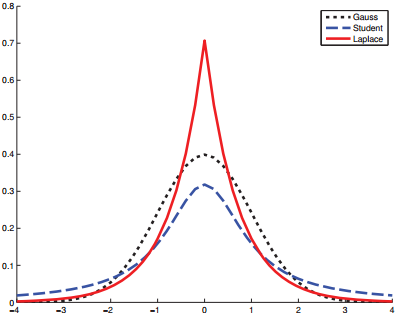
\includegraphics[scale=.70]{pdfs-for-NTL-a.png}} \\
\subfloat[]{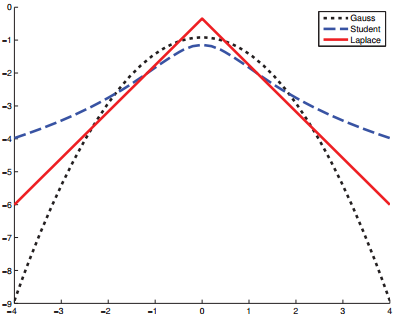
\includegraphics[scale=.70]{pdfs-for-NTL-b.png}}
\caption{(a) The pdf’s for a $\mathcal{N}(0,1)$, $\mathcal{T}(0,1,1)$ and $Lap(0,1/\sqrt{2})$. The mean is 0 and the variance is 1 for both the Gaussian and Laplace. The mean and variance of the Student is undefined when $\nu=1$.(b) Log of these pdf’s. Note that the Student distribution is not log-concave for any parameter value, unlike the Laplace distribution, which is always log-concave (and log-convex...) Nevertheless, both are unimodal.}
\label{fig:pdfs-for-NTL} 
\end{figure}

The variance is only defined if $\nu>2$. The mean is only defined if $\nu>1$.

As an illustration of the robustness of the Student distribution, consider Figure \ref{fig:robustness}. We see that the Gaussian is affected a lot, whereas the Student distribution hardly changes. This is because the Student has heavier tails, at least for small $\nu$(see Figure \ref{fig:pdfs-for-NTL}).

\begin{figure}[hbtp]
\centering
\subfloat[]{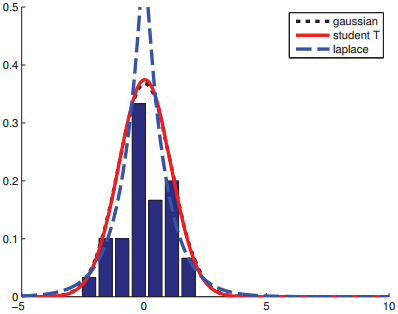
\includegraphics[scale=.70]{robustness-a.png}} \\
\subfloat[]{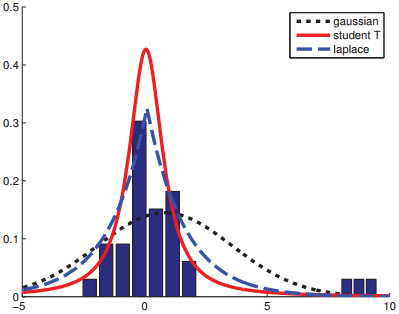
\includegraphics[scale=.70]{robustness-b.png}}
\caption{Illustration of the effect of outliers on fitting Gaussian, Student and Laplace distributions. (a) No outliers (the Gaussian and Student curves are on top of each other). (b) With outliers. We see that the Gaussian is more affected by outliers than the Student and Laplace distributions.}
\label{fig:robustness} 
\end{figure}

If $\nu=1$, this distribution is known as the \textbf{Cauchy} or \textbf{Lorentz} distribution. This is notable for having such heavy tails that the integral that defines the mean does not converge.

To ensure finite variance, we require $\nu>2$. It is common to use $\nu=4$, which gives good performance in a range of problems (Lange et al. 1989). For $\nu \gg 5$, the Student distribution rapidly approaches a Gaussian distribution and loses its robustness properties.


\subsection{The Laplace distribution}
\begin{table}
\caption{Summary of Laplace distribution.}
\centering
\begin{tabular}{cccccc}
\hline\noalign{\smallskip}
Written as & $f(x)$ & $\mathbb{E}[X]$ & mode & $\text{var}[X]$ \\
\noalign{\smallskip}\svhline\noalign{\smallskip}
$X \sim \text{Lap}(\mu,b)$ & $\dfrac{1}{2b}\exp\left(-\dfrac{|x-\mu|}{b}\right)$ & $\mu$ & $\mu$ & $2b^2$ \\
\noalign{\smallskip}\hline
\end{tabular}
\end{table}

Here $\mu$ is a location parameter and $b>0$ is a scale parameter. See Figure \ref{fig:pdfs-for-NTL} for a plot.

Its robustness to outliers is illustrated in Figure \ref{fig:robustness}. It also put mores probability density at 0 than the Gaussian. This property is a useful way to encourage sparsity in a model, as we will see in Section TODO.


\subsection{The gamma distribution}

\begin{table}
\caption{Summary of gamma distribution}
\centering
\begin{tabular}{ccccccc}
\hline\noalign{\smallskip}
Written as & $X$ & $f(x)$ & $\mathbb{E}[X]$ & mode & $\text{var}[X]$ \\
\noalign{\smallskip}\svhline\noalign{\smallskip}
$X \sim \text{Ga}(a,b)$ & $x \in \mathbb{R}^+$ & $\dfrac{b^a}{\Gamma(a)}x^{a-1}e^{-xb}$ & $\dfrac{a}{b}$ & $\dfrac{a-1}{b}$ & $\dfrac{a}{b^2}$ \\
\noalign{\smallskip}\hline
\end{tabular}
\end{table} 

Here $a>0$ is called the shape parameter and $b>0$ is called the rate parameter. See Figure \ref{fig:gamma-distribution} for some plots.

\begin{figure}[hbtp]
\centering
\subfloat[]{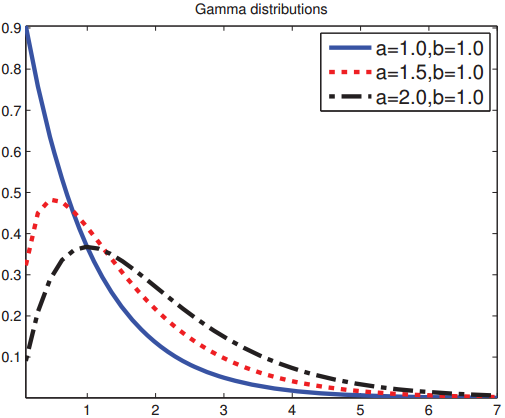
\includegraphics[scale=.50]{gamma-distribution-a.png}} \\
\subfloat[]{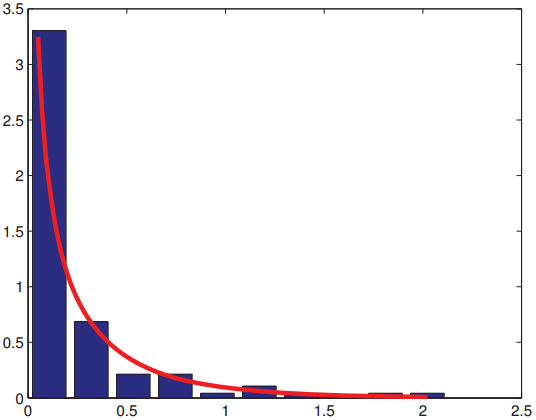
\includegraphics[scale=.50]{gamma-distribution-b.png}}
\caption{Some Ga$(a, b=1)$ distributions. If $a \leq 1$, the mode is at 0, otherwise it is $>0$.As we increase the rate $b$, we reduce the horizontal scale, thus squeezing everything leftwards and upwards. (b) An empirical pdf of some rainfall data, with a fitted Gamma distribution superimposed.}
\label{fig:gamma-distribution} 
\end{figure}


\subsection{The beta distribution}

\begin{table*}
\caption{Summary of Beta distribution}\label{tab:beta-distribution}
\centering
\begin{tabular}{ccccccc}
\hline\noalign{\smallskip}
Name & Written as & $X$ & $f(x)$ & $\mathbb{E}[X]$ & mode & $\text{var}[X]$ \\
\noalign{\smallskip}\svhline\noalign{\smallskip}
Beta distribution & $X \sim \text{Beta}(a,b)$ & $x \in [0,1]$ & $\dfrac{1}{B(a,b)}x^{a-1}(1-x)^{b-1}$ & $\dfrac{a}{a+b}$ & $\dfrac{a-1}{a+b-2}$ & $\dfrac{ab}{(a+b)^2(a+b+1)}$ \\
\noalign{\smallskip}\hline
\end{tabular}
\end{table*} 

Here $B(a, b)$is the beta function,
\begin{equation}
B(a,b) \triangleq \dfrac{\Gamma(a)\Gamma(b)}{\Gamma(a+b)}
\end{equation}

See Figure \ref{fig:beta-distribution} for plots of some beta distributions. We require  $a, b >0$ to ensure the distribution is integrable (i.e., to ensure $B(a, b)$ exists). If $a=b=1$, we get the uniform distirbution. If $a$ and $b$ are both less than 1, we get a bimodal distribution with “spikes” at 0 and 1; if $a$ and $b$ are both greater than 1, the distribution is unimodal.

\begin{figure}[hbtp]
\centering
    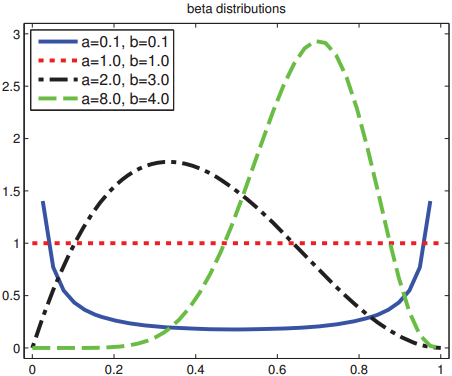
\includegraphics[scale=.60]{beta-distribution.png}
\caption{Some beta distributions.}
\label{fig:beta-distribution} 
\end{figure}


\subsection{Pareto distribution}

\begin{table*}
\caption{Summary of Pareto distribution}
\centering
\begin{tabular}{ccccccc}
\hline\noalign{\smallskip}
Name & Written as & $X$ & $f(x)$ & $\mathbb{E}[X]$ & mode & $\text{var}[X]$ \\
\noalign{\smallskip}\svhline\noalign{\smallskip}
Pareto distribution & $X \sim \text{Pareto}(k,m)$ & $x \geq m$ & $km^kx^{-(k+1)}\mathbb{I}(x \geq m)$ & $\dfrac{km}{k-1} \text{ if } k > 1$ & $m$ & $\dfrac{m^2k}{(k-1)^2(k-2)} \text{ if } k>2$ \\
\noalign{\smallskip}\hline
\end{tabular}
\end{table*} 

The \textbf{Pareto distribution} is used to model the distribution of quantities that exhibit \textbf{long tails}, also called \textbf{heavy tails}.

As $k \rightarrow \infty$, the distribution approaches $\delta(x-m)$. See Figure \ref{fig:Pareto-distribution}(a) for some plots. If we plot the distribution on a log-log scale, it forms a straight line, of the form $\log p(x)=a\log x+c$ for some constants $a$ and $c$. See Figure \ref{fig:Pareto-distribution}(b) for an illustration (this is known as a \textbf{power law}).

\begin{figure}[hbtp]
\centering
\subfloat[]{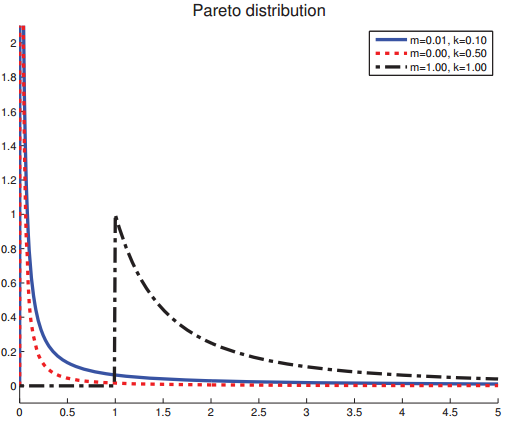
\includegraphics[scale=.50]{Pareto-distribution-a.png}} \\
\subfloat[]{\includegraphics[scale=.50]{Pareto-distribution-b.png}}
\caption{(a) The Pareto distribution Pareto$(x|m, k)$ for $m=1$. (b) The pdf on a log-log scale.}
\label{fig:Pareto-distribution} 
\end{figure}


\section{Joint probability distributions}
Given a \textbf{multivariate random variable} or \textbf{random vector} \footnote{\url{http://en.wikipedia.org/wiki/Multivariate_random_variable}} $X \in \mathbb{R}^D$, the \textbf{joint probability distribution}\footnote{\url{http://en.wikipedia.org/wiki/Joint_probability_distribution}} is a probability distribution that gives the probability that each of $X_1, X_2, \cdots,X_D$ falls in any particular range or discrete set of values specified for that variable. In the case of only two random variables, this is called a \textbf{bivariate distribution}, but the concept generalizes to any number of random variables, giving a \textbf{multivariate distribution}.

The joint probability distribution can be expressed either in terms of a \textbf{joint cumulative distribution function} or in terms of a \textbf{joint probability density function} (in the case of continuous variables) or \textbf{joint probability mass function} (in the case of discrete variables). 


\subsection{Covariance and correlation}
\begin{definition}
The \textbf{covariance} between two rv’s $X$ and $Y$ measures the degree to which $X$ and $Y$ are (linearly) related. Covariance is defined as
\begin{equation}
\begin{split}
\mathrm{cov}[X,Y] & \triangleq \mathbb{E}\left[(X-\mathbb{E}[X])(Y-\mathbb{E}[Y])\right] \\
         & =\mathbb{E}[XY]-\mathbb{E}[X]\mathbb{E}[Y]
\end{split}
\end{equation}
\end{definition}

\begin{definition}
If $X$ is a $D$-dimensional random vector, its \textbf{covariance matrix} is defined to be the following symmetric, positive definite matrix:
\begin{align}
\mathrm{cov}[X] & \triangleq \mathbb{E}\left[(X-\mathbb{E}[X])(X-\mathbb{E}[X])^T\right] \\
       &  = \left( \begin{array}{cccc}
           \text{var}[X_1] & \text{Cov}[X_1,X_2] & \cdots & \text{Cov}[X_1,X_D] \\
           \text{Cov}[X_2,X_1] & \text{var}[X_2] & \cdots & \text{Cov}[X_2,X_D] \\
		   \vdots & \vdots & \ddots & \vdots \\
           \text{Cov}[X_D,X_1] & \text{Cov}[X_D,X_2] & \cdots & \text{var}[X_D] \end{array} \right)
\end{align}
\end{definition}

\begin{definition}
The (Pearson) \textbf{correlation coefficient} between $X$ and $Y$ is defined as
\begin{equation}
\text{corr}[X,Y] \triangleq \dfrac{\text{Cov}[X,Y]}{\sqrt{\text{var}[X],\text{var}[Y]}}
\end{equation}
\end{definition}

A \textbf{correlation matrix} has the form
\begin{equation}
\mathbf{R} \triangleq \left( \begin{array}{cccc}
           \text{corr}[X_1,X_1] & \text{corr}[X_1,X_2] & \cdots & \text{corr}[X_1,X_D] \\
           \text{corr}[X_2,X_1] & \text{corr}[X_2,X_2] & \cdots & \text{corr}[X_2,X_D] \\
		   \vdots & \vdots & \ddots & \vdots \\
           \text{corr}[X_D,X_1] & \text{corr}[X_D,X_2] & \cdots & \text{corr}[X_D,X_D] \end{array} \right)
\end{equation}

The correlation coefficient can viewed as a degree of linearity between $X$ and $Y$, see Figure \ref{fig:Correlation-examples}.
\begin{figure*}[hbtp]
\centering
    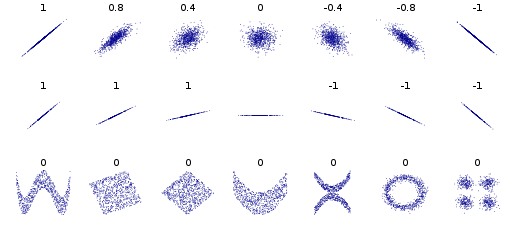
\includegraphics[scale=.80]{Correlation-examples.png}
\caption{Several sets of $(x, y)$ points, with the Pearson correlation coefficient of $x$ and $y$ for each set. Note that the correlation reflects the noisiness and direction of a linear relationship (top row), but not the slope of that relationship (middle), nor many aspects of nonlinear relationships (bottom). N.B.: the figure in the center has a slope of 0 but in that case the correlation coefficient is undefined because the variance of $Y$ is zero.Source:\url{http://en.wikipedia.org/wiki/Correlation}}
\label{fig:Correlation-examples} 
\end{figure*}

\textbf{Uncorrelated does not imply independent}. For example, let $X \sim U(-1,1)$ and $Y =X^2$. Clearly $Y$ is dependent on $X$(in fact, $Y$ is uniquely determined by $X$), yet one can show that corr$[X, Y]=0$. Some striking examples of this fact are shown in Figure \ref{fig:Correlation-examples}. This shows several data sets where there is clear dependence between $X$ and $Y$, and yet the correlation coefficient is 0. A more general measure of dependence between random variables is mutual information, see Section TODO.


\subsection{Multivariate Gaussian distribution}
\label{sec:MVN}
The \textbf{multivariate Gaussian} or \textbf{multivariate normal}(MVN) is the most widely used joint probability density function for continuous variables. We discuss MVNs in detail in Chapter 4; here we just give some definitions and plots.

The pdf of the MVN in $D$ dimensions is defined by the following:
\begin{equation}
\mathcal{N}(\vec{x}|\vec{\mu},\Sigma) \triangleq \dfrac{1}{(2\pi)^{D/2}|\Sigma|^{1/2}}\exp\left[-\dfrac{1}{2}(\vec{x}-\vec{\mu})^T\Sigma^{-1}(\vec{x}-\vec{\mu})\right]
\end{equation}
where $\vec{\mu}=\mathbb{E}[X] \in \mathbb{R}^D$ is the mean vector, and $\Sigma=\text{Cov}[X]$ is the $D \times D$ covariance matrix. The normalization constant $(2\pi)^{D/2}|\Sigma|^{1/2}$ just ensures that the pdf integrates to 1.

Figure \ref{fig:2d-Gaussions} plots some MVN densities in 2d for three different kinds of covariance matrices. A full covariance matrix has A $D(D+1)/2$ parameters (we divide by 2 since $\Sigma$ is symmetric). A diagonal covariance matrix has $D$ parameters, and has 0s in the off-diagonal terms. A spherical or isotropic covariance,$\Sigma=\sigma^2\vec{I}_D$, has one free parameter.

\begin{figure}[hbtp]
\centering
\subfloat[]{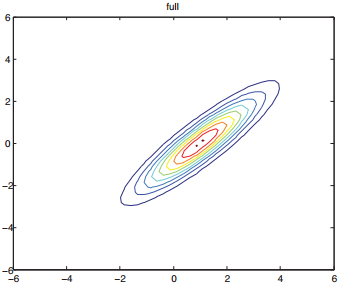
\includegraphics[scale=.60]{2d-Gaussions-a.png}} \\
\subfloat[]{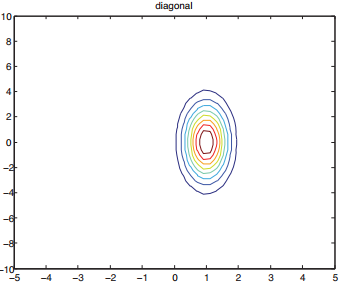
\includegraphics[scale=.60]{2d-Gaussions-b.png}} \\
\subfloat[]{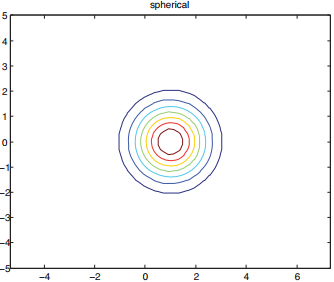
\includegraphics[scale=.60]{2d-Gaussions-c.png}} \\
\subfloat[]{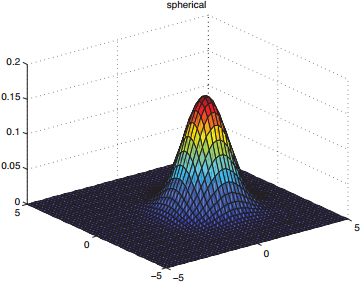
\includegraphics[scale=.60]{2d-Gaussions-d.png}}
\caption{We show the level sets for 2d Gaussians. (a) A full covariance matrix has elliptical contours.(b) A diagonal covariance matrix is an axis aligned ellipse. (c) A spherical covariance matrix has a circular shape. (d) Surface plot for the spherical Gaussian in (c).}
\label{fig:2d-Gaussions} 
\end{figure}


\subsection{Multivariate Student's t-distribution}
A more robust alternative to the MVN is the multivariate Student's t-distribution, whose pdf is given by
\begin{align}
& \mathcal{T}(x|\vec{\mu},\Sigma,\nu) \nonumber \\
& \triangleq \dfrac{\Gamma(\frac{\nu+D}{2})}{\Gamma(\frac{\nu}{2})}\dfrac{|\Sigma|^{-\frac{1}{2}}}{\left(\nu\pi\right)^{\frac{D}{2}}}\left[1+\dfrac{1}{\nu}\left(\vec{x}-\vec{\mu}\right)^T\Sigma^{-1}\left(\vec{x}-\vec{\mu}\right)\right]^{-\frac{\nu+D}{2}} \\
&= \dfrac{\Gamma(\frac{\nu+D}{2})}{\Gamma(\frac{\nu}{2})}\dfrac{|\Sigma|^{-\frac{1}{2}}}{\left(\nu\pi\right)^{\frac{D}{2}}}\left[1+\left(\vec{x}-\vec{\mu}\right)^T\vec{V}^{-1}\left(\vec{x}-\vec{\mu}\right)\right]^{-\frac{\nu+D}{2}}
\end{align}
where $\Sigma$ is called the scale matrix (since it is not exactly the covariance matrix) and $\vec{V}=\nu\Sigma$. This has fatter tails than a Gaussian. The smaller $\nu$ is, the fatter the tails. As $\nu \rightarrow \infty$, the distribution tends towards a Gaussian. The distribution has the following properties
\begin{equation}
\text{mean}=\vec{\mu} \text{ , mode}=\vec{\mu} \text{ , Cov}= \dfrac{\nu}{\nu-2}\Sigma
\end{equation}


\subsection{Dirichlet distribution}
A multivariate generalization of the beta distribution is the \textbf{Dirichlet distribution}, which has
support over the probability simplex, defined by
\begin{equation}
S_K=\left\{\vec{x}:0 \leq x_k \leq 1,\sum\limits_{k=1}^K x_k=1\right\}
\end{equation}

The pdf is defined as follows:
\begin{equation}
\text{Dir}(\vec{x}|\vec{\alpha}) \triangleq \dfrac{1}{B(\vec{\alpha})}\prod\limits_{k=1}^K x_k^{\alpha_k-1}\mathbb{I}(\vec{x} \in S_K)
\end{equation}
where $B(\alpha_1,\alpha_2,\cdots,\alpha_K)$ is the natural generalization of the beta function to $K$ variables:
\begin{equation}
B(\alpha) \triangleq \dfrac{\prod_{k=1}^K \Gamma(\alpha_k)}{\Gamma(\alpha_0)} \text{ where } \alpha_0 \triangleq \sum_{k=1}^K \alpha_k
\end{equation}

Figure \ref{fig:3d-Dirichlet} shows some plots of the Dirichlet when $K=3$, and Figure \ref{fig:5d-Dirichlet} for some sampled probability vectors. We see that $\alpha_0$ controls the strength of the distribution (how peaked it is), and theαkcontrol where the peak occurs. For example, Dir$(1,1,1)$ is a uniform distribution, Dir$(2,2,2)$ is a broad distribution centered at $(1/3,1/3,1/3)$, and Dir$(20,20,20)$ is a narrow distribution centered at $(1/3,1/3,1/3)$.If $\alpha_k < 1$ for all $k$, we get “spikes” at the corner of the simplex.

\begin{figure}[hbtp]
\centering
\subfloat[]{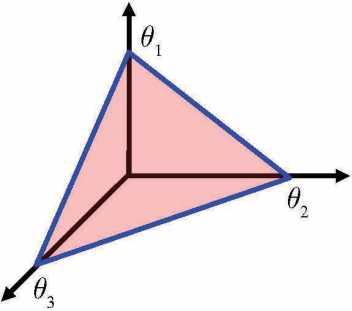
\includegraphics[scale=.50]{3d-Dirichlet-a.png}} \\
\subfloat[]{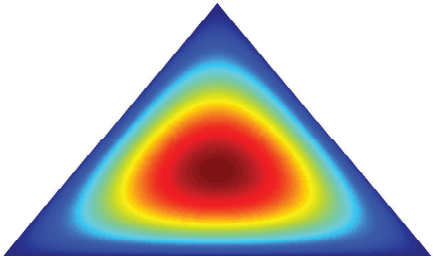
\includegraphics[scale=.60]{3d-Dirichlet-b.png}} \\
\subfloat[]{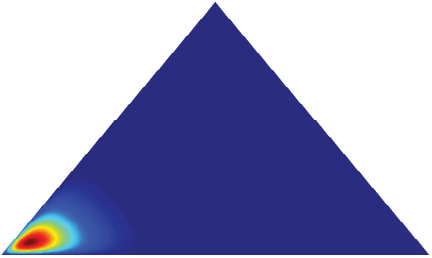
\includegraphics[scale=.60]{3d-Dirichlet-c.png}} \\
\subfloat[]{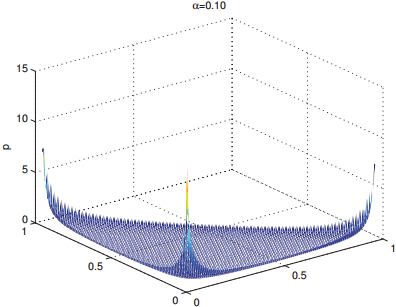
\includegraphics[scale=.60]{3d-Dirichlet-d.png}}
\caption{(a) The Dirichlet distribution when $K=3$ defines a distribution over the simplex, which can be represented by the triangular surface. Points on this surface satisfy $0 \leq \theta_k \leq 1$ and $\sum_{k=1}^K \theta_k=1$. (b) Plot of the Dirichlet density when $\vec{\alpha}=(2,2,2)$. (c) $\vec{\alpha}=(20,2,2)$.}
\label{fig:3d-Dirichlet} 
\end{figure}

\begin{figure}[hbtp]
\centering
\subfloat[$\vec{\alpha}=(0.1,\cdots,0.1)$. This results in very sparse distributions, with many 0s.]{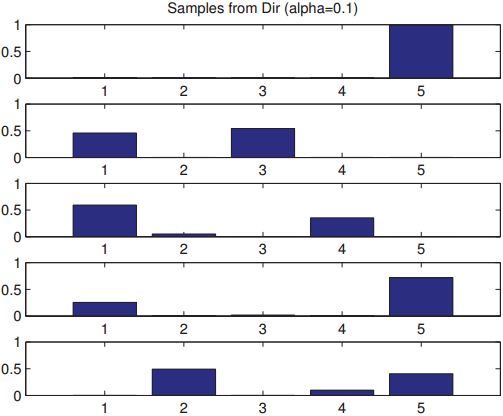
\includegraphics[scale=.50]{5d-Dirichlet-a.png}} \\
\subfloat[$\vec{\alpha}=(1,\cdots,1)$. This results in more uniform (and dense) distributions.]{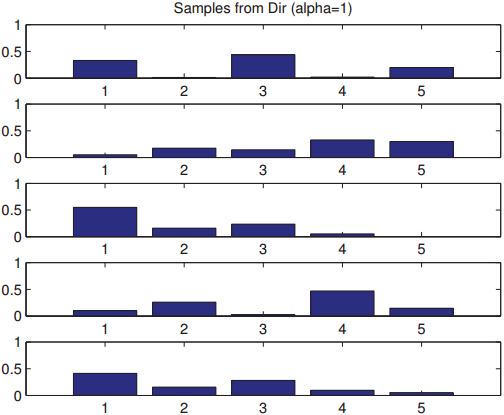
\includegraphics[scale=.50]{5d-Dirichlet-b.png}}
\caption{Samples from a 5-dimensional symmetric Dirichlet distribution for different parameter values.} 
\label{fig:5d-Dirichlet} 
\end{figure}

For future reference, the distribution has these properties
\begin{equation}\label{eqn:Dirichlet-properties}
\mathbb{E}(x_k)=\dfrac{\alpha_k}{\alpha_0} \text{, mode}[x_k]=\dfrac{\alpha_k-1}{\alpha_0-K} \text{, var}[x_k]=\dfrac{\alpha_k(\alpha_0-\alpha_k)}{\alpha_0^2(\alpha_0+1)}
\end{equation}


\section{Transformations of random variables}
If $\vec{x} \sim P()$ is some random variable, and $\vec{y}=f(\vec{x})$, what is the distribution of $Y$? This is the question we address in this section.


\subsection{Linear transformations}
Suppose $g()$ is a linear function: 
\begin{equation}
g(\vec{x})=A\vec{x}+b
\end{equation}

First, for the mean, we have
\begin{equation}
\mathbb{E}[\vec{y}]=\mathbb{E}[A\vec{x}+b]=A\mathbb{E}[\vec{x}]+b
\end{equation}
this is called the \textbf{linearity of expectation}.

For the covariance, we have
\begin{equation}
\text{Cov}[\vec{y}]=\text{Cov}[A\vec{x}+b]=A\Sigma A^T
\end{equation}


\subsection{General transformations}
\label{sec:General-transformations}
If $X$ is a discrete rv, we can derive the pmf for $y$ by simply summing up the probability mass for all the $x$’s such that $f(x)=y$:
\begin{equation}\label{eqn:transformation-discrete}
p_Y(y)=\sum\limits_{x:g(x)=y}p_X(x)
\end{equation}

If $X$ is continuous, we cannot use Equation \ref{eqn:transformation-discrete} since $p_X(x)$ is a density, not a pmf, and we cannot sum up densities. Instead, we work with cdf’s, and write
\begin{equation}
F_Y(y)=P(Y \leq y)=P(g(X) \leq y)=\int\limits_{g(X) \leq y} f_X(x)\mathrm{d}x
\end{equation}

We can derive the pdf of $Y$ by differentiating the cdf:
\begin{equation}\label{eqn:General-transformations}
f_Y(y)=f_X(x)|\dfrac{dx}{dy}|
\end{equation}

This is called \textbf{change of variables} formula. We leave the proof of this as an exercise. 

For example, suppose $X \sim U(−1,1)$, and $Y=X^2$. Then $p_Y(y)=\dfrac{1}{2}y^{-\frac{1}{2}}$.


\subsubsection{Multivariate change of variables *}
Let $f$ be a function $f:\mathbb{R}^n \rightarrow \mathbb{R}^n$, and let $\vec{y}=f(\vec{x})$. Then its Jacobian matrix $\vec{J}$ is given by
\begin{equation}
\vec{J}_{\vec{x} \rightarrow \vec{y}} \triangleq \frac{\partial \vec{y}}{\partial \vec{x}} \triangleq \left(\begin{array}{ccc}
\frac{\partial y_1}{\partial x_1} & \cdots & \frac{\partial y_1}{\partial x_n} \\
\vdots & \vdots & \vdots \\
\frac{\partial y_n}{\partial x_1} & \cdots & \frac{\partial y_n}{\partial x_n}
\end{array}\right)
\end{equation}
$|\mathrm{det}(\vec{J})|$ measures how much a unit cube changes in volume when we apply $f$.

If $f$ is an invertible mapping, we can define the pdf of the transformed variables using the Jacobian of the inverse mapping $\vec{y} \rightarrow \vec{x}$:
\begin{equation}\label{eqn:Multivariate-transformation}
p_y(\vec{y})=p_x(\vec{x})|\mathrm{det}(\frac{\partial \vec{x}}{\partial \vec{y}})|=p_x(\vec{x})|\mathrm{det}(\vec{J}_{\vec{y} \rightarrow \vec{x}})|
\end{equation}


\subsection{Central limit theorem}
Given $N$ random variables $X_1,X_2,\cdots,X_N$, each variable is \textbf{independent and identically distributed}\footnote{\url{http://en.wikipedia.org/wiki/Independent_identically_distributed}}(\textbf{iid} for short), and each has the same mean $\mu$ and variance $\sigma^2$, then
\begin{equation}
\dfrac{\sum\limits_{i=1}^n X_i-N\mu}{\sqrt{N}\sigma} \sim \mathcal{N}(0,1)
\end{equation}
this can also be written as
\begin{equation}
\dfrac{\bar{X}-\mu}{\sigma/\sqrt{N}} \sim \mathcal{N}(0,1) \quad \text{, where } \bar{X} \triangleq \dfrac{1}{N}\sum\limits_{i=1}^n X_i
\end{equation}


\section{Monte Carlo approximation}
\label{sec:Monte-Carlo-approximation}
In general, computing the distribution of a function of an rv using the change of variables formula can be difficult. One simple but powerful alternative is as follows. First we generate $S$ samples from the distribution, call them $x_1,\cdots,x_S$. (There are many ways to generate such samples; one popular method, for high dimensional distributions, is called Markov chain Monte Carlo or MCMC; this will be explained in Chapter TODO.) Given the samples, we can approximate the distribution of $f(X)$ by using the empirical distribution of $\left\{f(x_s)\right\}_{s=1}^S$. This is called a \textbf{Monte Carlo approximation}\footnote{\url{http://en.wikipedia.org/wiki/Monte_Carlo_method}}, named after a city in Europe known for its plush gambling casinos.

We can use Monte Carlo to approximate the expected value of any function of a random variable. We simply draw samples, and then compute the arithmetic mean of the function applied to the samples. This can be written as follows:
\begin{equation}
\mathbb{E}[g(X)]=\int g(x)p(x)\mathrm{d}x \approx \dfrac{1}{S}\sum\limits_{s=1}^S f(x_s)
\end{equation}
where $x_s \sim p(X)$.

This is called \textbf{Monte Carlo integration}\footnote{\url{http://en.wikipedia.org/wiki/Monte_Carlo_integration}}, and has the advantage over numerical integration (which is based on evaluating the function at a fixed grid of points) that the function is only evaluated in places where there is non-negligible probability.


\section{Information theory}

\subsection{Entropy}
\label{sec:Entropy}
The entropy of a random variable $X$ with distribution $p$, denoted by $\mathbb{H}(X)$ or sometimes $\mathbb{H}(p)$, is a measure of its uncertainty. In particular, for a discrete variable with $K$ states, it is defined by
\begin{equation}
\mathbb{H}(X) \triangleq -\sum\limits_{k=1}^{K}{p(X=k)\log_2p(X=k)}
\end{equation}

Usually we use log base 2, in which case the units are called \textbf{bits}(short for binary digits). If we use log base $e$ , the units are called \textbf{nats}. 

The discrete distribution with maximum entropy is the uniform distribution (see Section XXX for a proof). Hence for a K-ary random variable, the entropy is maximized if $p(x = k)=1/K$; in this case, $\mathbb{H}(X)=\log_2K$. 

Conversely, the distribution with minimum entropy (which is zero) is any \textbf{delta-function} that puts all its mass on one state. Such a distribution has no uncertainty.


\subsection{KL divergence}
One way to measure the dissimilarity of two probability distributions, $p$ and $q$ , is known as the \textbf{Kullback-Leibler divergence}(\textbf{KL divergence})or \textbf{relative entropy}. This is defined as follows:
\begin{equation}
\mathbb{KL}(P||Q) \triangleq 
\sum\limits_{x}{p(x)\log_2\dfrac{p(x)}{q(x)}}
\end{equation}
where the sum gets replaced by an integral for pdfs\footnote{The KL divergence is not a distance, since it is asymmetric. One symmetric version of the KL divergence is the \textbf{Jensen-Shannon divergence}, defined as $JS(p_1,p_2)=0.5\mathbb{KL}(p_1||q)+0.5\mathbb{KL}(p_2||q)$,where $q=0.5p_1+0.5p_2$}. The KL divergence is only defined if P and Q both sum to 1 and if $q(x)=0$ implies $p(x)=0$ for all $x$(absolute continuity). If the quantity  $0\ln0$ appears in the formula, it is interpreted as zero because $\lim\limits_{x \to 0}x\ln x$. We can rewrite this as
\begin{equation}\begin{split}
\mathbb{KL}(p||q) & \triangleq \sum\limits_{x}{p(x)\log_2p(x)}-\sum\limits_{k=1}^{K}{p(x)\log_2q(x)} \\
    & =\mathbb{H}(p)-\mathbb{H}(p,q)
\end{split}\end{equation}
where $\mathbb{H}(p,q)$ is called the \textbf{cross entropy},
\begin{equation}\label{eqn:cross-entropy}
\mathbb{H}(p,q)=\sum\limits_{x}{p(x)\log_2q(x)}
\end{equation}

One can show (Cover and Thomas 2006) that the cross entropy is the average number of bits needed to encode data coming from a source with distribution $p$ when we use model $q$ to define our codebook. Hence the “regular” entropy $\mathbb{H}(p)=\mathbb{H}(p,p)$, defined in section \S \ref{sec:Entropy},is the expected number of bits if we use the true model, so the KL divergence is the diference between these. In other words, the KL divergence is the average number of \emph{extra} bits needed to encode the data, due to the fact that we used distribution $q$ to encode the data instead of the true distribution $p$.

The “extra number of bits” interpretation should make it clear that $\mathbb{KL}(p||q) \geq 0$, and that the KL is only equal to zero if $q = p$. We now give a proof of this important result.

\begin{theorem}
(\textbf{Information inequality}) $\mathbb{KL}(p||q) \geq 0 \text{ with equality iff } p=q$.
\end{theorem}

One important consequence of this result is that \emph{the discrete distribution with the maximum
entropy is the uniform distribution}.


\subsection{Mutual information}
\label{sec:Mutual-information}
\begin{definition}
\textbf{Mutual information} or \textbf{MI}, is defined as follows:
\begin{equation}\begin{split}
\mathbb{I}(X;Y) & \triangleq \mathbb{KL}(P(X,Y)||P(X)P(X)) \\
    & =\sum\limits_x\sum\limits_yp(x,y)\log\dfrac{p(x,y)}{p(x)p(y)}
\end{split}\end{equation}
We have $\mathbb{I}(X;Y) \geq 0$ with equality if $P(X,Y)=P(X)P(Y)$. That is, the MI is zero if the variables are independent.
\end{definition}

To gain insight into the meaning of MI, it helps to re-express it in terms of joint and conditional entropies. One can show that the above expression is equivalent to the following:
\begin{eqnarray}
\mathbb{I}(X;Y)&=&\mathbb{H}(X)-\mathbb{H}(X|Y)\\
               &=&\mathbb{H}(Y)-\mathbb{H}(Y|X)\\
               &=&\mathbb{H}(X)+\mathbb{H}(Y)-\mathbb{H}(X,Y)\\
               &=&\mathbb{H}(X,Y)-\mathbb{H}(X|Y)-\mathbb{H}(Y|X)
\end{eqnarray}
where $\mathbb{H}(X)$ and $\mathbb{H}(Y)$ are the \textbf{marginal entropies}, $\mathbb{H}(X|Y)$ and $\mathbb{H}(Y|X)$ are the \textbf{conditional entropies}, and $\mathbb{H}(X,Y)$ is the \textbf{joint entropy} of $X$ and $Y$, see Fig. \ref{fig:mi}\footnote{\url{http://en.wikipedia.org/wiki/Mutual_information}}.

\begin{figure}[hbtp]
\centering
    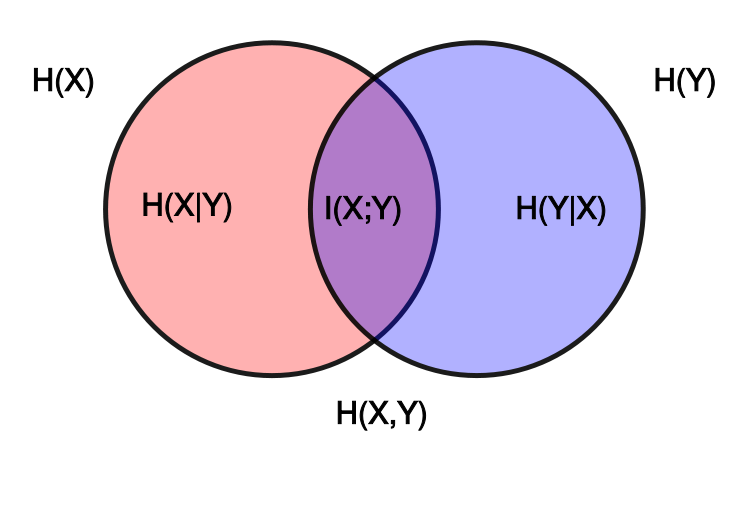
\includegraphics[scale=.25]{mutual-information.png}
\caption{Individual $\mathbb{H}(X),\mathbb{H}(Y)$, joint $\mathbb{H}(X,Y)$, and conditional entropies for a pair of correlated subsystems $X,Y$ with mutual information $\mathbb{I}(X;Y)$.}
\label{fig:mi} 
\end{figure}

Intuitively, we can interpret the MI between $X$ and $Y$ as the reduction in uncertainty about $X$ after observing $Y$, or, by symmetry, the reduction in uncertainty about $Y$ after observing $X$.

A quantity which is closely related to MI is the \textbf{pointwise mutual information} or \textbf{PMI}. For two events (not random variables) $x$ and $y$, this is defined as
\begin{equation}
PMI(x,y) \triangleq \log\dfrac{p(x,y)}{p(x)p(y)}=\log\dfrac{p(x|y)}{p(x)}=\log\dfrac{p(y|x)}{p(y)}
\end{equation}

This measures the discrepancy between these events occuring together compared to what would be expected by chance. Clearly the MI of $X$ and $Y$ is just the expected value of the PMI. Interestingly, we can rewrite the PMI as follows:
\begin{equation}
PMI(x,y)=\log\dfrac{p(x|y)}{p(x)}=\log\dfrac{p(y|x)}{p(y)}
\end{equation}

This is the amount we learn from updating the prior $p(x)$ into the posterior $p(x|y)$ , or equivalently, updating the prior $p(y)$ into the posterior $p(y |x)$ .
\chapter{Perceptron}
\label{chap:Perceptron}

\section{Model}
\begin{equation}
\mathcal{H}:f(\vec{x})=\text{sign}(\vec{w}\vec{x}+b)
\end{equation}
where $\text{sign}(x)=\begin{cases}+1, & x \geq 0\\-1, & x<0\\\end{cases}$, see Fig. ~\ref{fig:perceptron}\footnote{\url{https://en.wikipedia.org/wiki/Perceptron}}.
\begin{figure}[hbtp]
\centering
    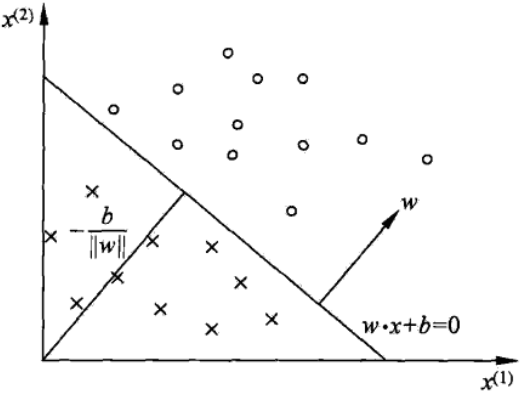
\includegraphics[scale=.50]{figures/perceptron.png}
\caption{Perceptron}
\label{fig:perceptron} 
\end{figure}

Perceptron is a binary linear classifier, which is a discriminant model.

\section{Strategy}
\begin{eqnarray}
L(\vec{w},b)&=&-y_i(\vec{wx}_i+b)\\
R_{emp}(f)&=&-\sum\limits_i y_i(\vec{wx}_i+b)\\
\end{eqnarray}

\section{Learning algorithm}
\subsection{Primal form}
Stochastic gradient descent, the pseudo code is as follows:
\begin{algorithm}[htbp]
    %\SetAlgoLined
    \SetAlgoNoLine
  
    $\vec{w} \leftarrow 0;\; b \leftarrow 0;\; k \leftarrow 0$\;
    \While{no mistakes made within the for loop}{
        \For{$i\leftarrow 1$ \KwTo $N$}{
			\If{$y_i(\vec{w}^T\vec{x}_i+b) \leq 0$}{
				$\vec{w} \leftarrow \vec{w}+\eta y_i \vec{x}_i$\;
				$b \leftarrow b+\eta y_i$\;
				$k \leftarrow k+1$\;
			}
		}
    }
\caption{Perceptron learning algorithm, primal form}
\end{algorithm}

\subsection{Convergency}
\begin{theorem}
(\textbf{Novikoff}) If traning data set $\mathcal{D}$ is linearly separable, then
\begin{enumerate}
\item There exists a hyperplane denoted as $\widehat{\vec{w}}_{opt} \cdot \vec{x}+b_{opt}=0$ which can correctly seperate all samples, and $\exists\gamma>0,\forall i, y_i(\vec{w}_{opt} \cdot \vec{x}_i+b_{opt}) \geq \gamma$
\item $k \leq \left(\dfrac{R}{\gamma}\right)^2$, where $R=\max\limits_{1 \leq i \leq N} \abs{\abs{\widehat{\vec{x}}_i}}$
\end{enumerate}
\end{theorem}

\begin{proof}
(1) let $\gamma=\min\limits_{i} y_i(\vec{w}_{opt} \cdot \vec{x}_i+b_{opt})$, then we get $y_i(\vec{w}_{opt} \cdot \vec{x}_i+b_{opt}) \geq \gamma$.

(2) The algorithm start from $\widehat{\vec{x}_0}=0$, if a instance is misclassified, then update the weight. Let $\widehat{\vec{w}_{k-1}}$ denotes the extended weight before the k-th misclassified instance, then we can get
\begin{eqnarray}
y_i(\widehat{\vec{w}}_{k-1} \cdot \widehat{\vec{x}_i})&=&y_i(\vec{w}_{k-1} \cdot \vec{x}_i+b_{k-1}) \leq 0\\
\widehat{\vec{w}}_k&=&\widehat{\vec{w}}_{k-1}+\eta y_i \widehat{\vec{x}_i}
\end{eqnarray}

We could infer the following two equations, the proof procedure are omitted.
\begin{enumerate}
\item $\widehat{\vec{w}}_k \cdot \widehat{\vec{w}}_{opt} \geq k\eta\gamma$
\item $\abs{\abs{\widehat{\vec{w}}_k}}^2 \leq k\eta^2R^2$
\end{enumerate}

From above two equations we get
\begin{eqnarray}
\nonumber k\eta\gamma & \leq & \widehat{\vec{w}}_k \cdot \widehat{\vec{w}}_{opt} \leq \abs{\abs{\widehat{\vec{w}}_k}}\abs{\abs{\widehat{\vec{w}}_{opt}}} \leq \sqrt k \eta R \\
\nonumber k^2\gamma^2 & \leq & kR^2 \\
\nonumber \text{i.e. } k & \leq & \left(\dfrac{R}{\gamma}\right)^2
\end{eqnarray}
\end{proof}

\subsection{Dual form}
\begin{eqnarray}
\vec{w}&=&\sum\limits_{i=1}^{N} \alpha_iy_i\vec{x}_i \\
b&=&\sum\limits_{i=1}^{N} \alpha_iy_i \\
f(\vec{x})&=&\text{sign}\left(\sum\limits_{j=1}^{N} \alpha_jy_j\vec{x}_j \cdot \vec{x}+b\right)
\end{eqnarray}

\begin{algorithm}[htbp]
    %\SetAlgoLined
    \SetAlgoNoLine
  
    $\vec{\alpha} \leftarrow 0;\; b \leftarrow 0;\; k \leftarrow 0$\;
    \While{no mistakes made within the for loop}{
        \For{$i\leftarrow 1$ \KwTo $N$}{
			\If{$y_i\left(\sum\limits_{j=1}^{N} \alpha_jy_j\vec{x}_j \cdot \vec{x}_i+b\right) \leq 0$}{
				$\vec{\alpha} \leftarrow \vec{\alpha}+\eta$\;
				$b \leftarrow b+\eta y_i$\;
				$k \leftarrow k+1$\;
			}
		}
    }
\caption{Perceptron learning algorithm, dual form}
\end{algorithm}
\chapter{K-Nearest Neighbors}


\section{Representation}

\begin{equation}
y=f(\vec{x})=\arg\min_{c}{\sum\limits_{\vec{x}_i \in N_k(\vec{x})} \mathbb{I}(y_i=c)}
\end{equation}
where $N_k(\vec{x})$ is the set of k points that are closest to point $\vec{x}$.

Usually use \textbf{k-d tree} to accelerate the process of finding k nearest points.


\section{Evaluation}
No training is needed.

\section{Optimization}
No training is needed.

\chapter{K-Means Clustering}


\section{Representation}
\begin{equation}
y_j=k \text{ if } \|\vec{x}_j-\vec{\mu}_k\|_2^2 \text{ is minimal}
\end{equation}
where $\vec{\mu}_k$ \ is\ the centroid of cluster k.


\section{Evaluation}
\begin{equation}
\arg\min\limits_{\vec{\mu}} \sum_{j=1}^N {\sum_{k=1}^K}\gamma_{jk}{\|\vec{x}_j-\vec{\mu}_k\|_2^2}
\end{equation}

The hidden variable is $\gamma_{jk}$, which's meanining is:
\begin{equation} \nonumber
\gamma_{jk}=\begin{cases}
1, & \text{if } \|\vec{x}_j-\vec{\mu}_k\|_2 \text{ is minimal for } \vec{\mu}_k \\
0, & \text{otherwise}
\end{cases}
\end{equation}


\section{Optimization}
E-Step:
\begin{equation}
\gamma_{jk}^{(i+1)}=\begin{cases} 
1, & \text{if } \|\vec{x}_j-\vec{\mu}_k^{(i)}\|_2 \text{ is minimal for } \vec{\mu}_k^{(i)} \\ 
0, & \text{otherwise}
\end{cases}
\end{equation}

M-Step:
\begin{equation}
\vec{\mu}_{k}^{(i+1)}= \frac{\sum_{j=1}^N{\gamma_{jk}^{(i+1)}\vec{x}_j}}{\sum \gamma_{jk}^{(i+1)}}
\end{equation}


\section{Reference}
1. cheat-sheet: Algorithm for supervised and unsupervised learning by Emanuel Ferm http://t.cn/hD0Stf

\chapter{Naive Bayes}

\chapter{Decision Tree}

\chapter{Linear Regression}


\section{Introduction}
Linear regression is the “work horse” of statistics and (supervised) machine learning. When augmented with kernels or other forms of basis function expansion, it can model also nonlinear relationships. And when the Gaussian output is replaced with a Bernoulli or multinoulli distribution, it can be used for classification, as we will see below. So it pays to study this model in detail.


\section{Representation}
Linear regression is a model of the form
\begin{equation}
p(y|\vec{x},\vec{\theta})=\mathcal{N}(y|\vec{w}^T\vec{x}, \sigma^2)
\end{equation}
where $\vec{w}$ and $\vec{x}$ are extended vectors, $\vec{x}=(1,x)$, $\vec{w}=(b,w)$.

Linear regression can be made to model non-linear relationships by replacing $\vec{x}$ with some non-linear function of the inputs, $\phi(\vec{x})$ \begin{equation}
p(y|\vec{x},\vec{\theta})=\mathcal{N}(y|\vec{w}^T\phi(\vec{x}), \sigma^2)
\end{equation}

This is known as \textbf{basis function expansion}. (Note that the model is still linear in the parameters $\vec{w}$, so it is still called linear regression; the importance of this will become clear below.) A simple example are polynomial basis functions, where the model has the form
\begin{equation}
\phi(x)=(1, x, \cdots, x^d)
\end{equation}



\section{MLE}
Instead of maximizing the log-likelihood, we can equivalently minimize the \textbf{negative log likelihood} or \textbf{NLL}:
\begin{equation}
\text{NLL}(\vec{\theta}) \triangleq -\ell(\vec{\theta})=-\log(\mathcal{D}|\vec{\theta})
\end{equation}

The NLL formulation is sometimes more convenient, since many optimization software packages are designed to find the minima of functions, rather than maxima.

Now let us apply the method of MLE to the linear regression setting. Inserting the definition of the Gaussian into the above, we find that the log likelihood is given by
\begin{align}
\ell(\vec{\theta})& =\sum\limits_{i=1}^N \log\left[\dfrac{1}{\sqrt{2\pi}\sigma}\exp\left(-\dfrac{1}{2\sigma^2}(y_i-\vec{w}^T\vec{x}_i)^2\right)\right] \\
     & =-\dfrac{1}{2\sigma^2}\text{RSS}(\vec{w})-\dfrac{\vec{w}}{2}\log(2\pi\sigma^2)
\end{align}

RSS stands for \textbf{residual sum of squares} and is defined by
\begin{equation}
\text{RSS}(\vec{w}) \triangleq \sum\limits_{i=1}^N (y_i-\vec{w}^T\vec{x}_i)^2
\end{equation}

We see that the MLE for $\vec{w}$ is the one that minimizes the RSS, so this method is known as \textbf{least squares}.

Let's drop constants wrt $\vec{w}$ and NLL can be written as
\begin{equation}
\text{NLL}(\vec{w}) = \dfrac{1}{2}\sum\limits_{i=1}^N (y_i-\vec{w}^T\vec{x}_i)^2
\end{equation}

There two ways to minimize NLL$(\vec{w})$.


\subsection{OLS}
Define $\vec{y}=(y_1,y_2,\cdots,y_N)$, $\vec{X}=\left(\begin{array}{c}\vec{x}_1^T \\ \vec{x}_2^T \\ \vdots \\ \vec{x}_N^T\end{array}\right)$, then NLL$(\vec{w})$ can be written as
\begin{equation}
\text{NLL}(\vec{w})=\dfrac{1}{2}(\vec{y}-\vec{X}\vec{w})^T(\vec{y}-\vec{X}\vec{w})
\end{equation}

When $\mathcal{D}$ is small(for example, $N < 1000$), we can use the following equation to compute \vec{w} directly
\begin{equation}
\hat{\vec{w}}_{\mathrm{OLS}}=(\vec{X}^T\vec{X})^{-1}\vec{X}^T\vec{y}
\end{equation}

The corresponding solution $\hat{\vec{w}}_{\mathrm{OLS}}$ to this linear system of equations is called the \textbf{ordinary least squares} or \textbf{OLS} solution.

\begin{proof}
We now state without proof some facts of matrix derivatives (we won’t need all of these at this section).
\begin{eqnarray}
trA &\triangleq& \sum\limits_{i=1}^n A_{ii} \nonumber \\
\frac{\partial}{\partial A}AB &=& B^T \\
\frac{\partial}{\partial A^T}f(A) &=& \left[\frac{\partial}{\partial A}f(A)\right]^T \label{eqn:matrix-1} \\
\frac{\partial}{\partial A}ABA^TC &=& CAB+C^TAB^T \label{eqn:matrix-2} \\
\frac{\partial}{\partial A}|A| &=& |A|(A^{-1})^T
\end{eqnarray}

Then,
\begin{eqnarray*}
\text{NLL}(\vec{w}) &=& \frac{1}{2N}(\vec{X}\vec{w}-\vec{y})^T(\vec{X}\vec{w}-\vec{y}) \\
\frac{\partial \text{NLL}}{\vec{w}} &=& \frac{1}{2} \frac{\partial}{\vec{w}} (\vec{w}^T\vec{X}^T\vec{X}\vec{w}-\vec{w}^T\vec{X}^T\vec{y}-\vec{y}^T\vec{X}\vec{w}+\vec{y}^T\vec{y}) \\
                           &=& \frac{1}{2} \frac{\partial}{\vec{w}} (\vec{w}^T\vec{X}^T\vec{X}\vec{w}-\vec{w}^T\vec{X}^T\vec{y}-\vec{y}^T\vec{X}\vec{w}) \\
						   &=& \frac{1}{2} \frac{\partial}{\vec{w}} tr(\vec{w}^T\vec{X}^T\vec{X}\vec{w}-\vec{w}^T\vec{X}^T\vec{y}-\vec{y}^T\vec{X}\vec{w}) \\
						   &=& \frac{1}{2} \frac{\partial}{\vec{w}} (tr\vec{w}^T\vec{X}^T\vec{X}\vec{w}-2tr\vec{y}^T\vec{X}\vec{w})
\end{eqnarray*}

Combining Equations \eqref{eqn:matrix-1} and \eqref{eqn:matrix-2}, we find that 
\begin{equation*}
\frac{\partial}{\partial A^T}ABA^TC = B^TA^TC^T+BA^TC
\end{equation*}

Let $A^T=\vec{w}, B=B^T=\vec{X}^T\vec{X}$, and $C=I$, Hence,
\begin{eqnarray}
\frac{\partial \text{NLL}}{\vec{w}} &=& \frac{1}{2} (\vec{X}^T\vec{X}\vec{w}+\vec{X}^T\vec{X}\vec{w} -2\vec{X}^T\vec{y}) \nonumber \\
						   &=& \frac{1}{2} (\vec{X}^T\vec{X}\vec{w} - \vec{X}^T\vec{y}) \nonumber \\
\frac{\partial \text{NLL}}{\vec{w}} &=& 0 \Rightarrow \vec{X}^T\vec{X}\vec{w} - \vec{X}^T\vec{y} =0 \nonumber \\
\vec{X}^T\vec{X}\vec{w} &=& \vec{X}^T\vec{y} \label{eqn:normal-equation} \\
\hat{\vec{w}}_{\mathrm{OLS}} &=& (\vec{X}^T\vec{X})^{-1}\vec{X}^T\vec{y} \nonumber
\end{eqnarray}
\end{proof}

Equation \eqref{eqn:normal-equation} is known as the \textbf{normal equation}.


\subsubsection{Geometric interpretation}

See Figure \ref{fig:graphical-interpretation-of-OLS}.
\begin{figure}[hbtp]
\centering
    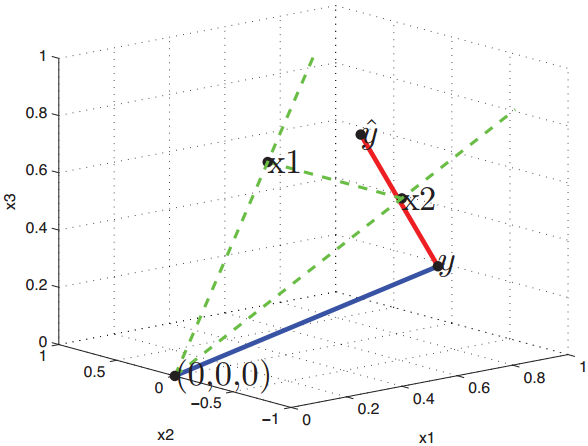
\includegraphics[scale=.60]{graphical-interpretation-of-OLS.png}
\caption{Graphical interpretation of least squares for $N=3$ examples and $D=2$ features. $\tilde{\vec{x}}_1$ and $\tilde{\vec{x}}_2$˜ are vectors in $\mathbb{R}^3$; together they define a 2D plane. $\vec{y}$ is also a vector in $\mathbb{R}^3$ but does not lie on this 2D plane. The orthogonal projection of $\vec{y}$ onto this plane is denoted $\hat{\vec{y}}$. The red line from $\vec{y}$ to $\hat{\vec{y}}$ is the residual, whose norm we want to minimize. For visual clarity, all vectors have been converted to unit norm.}
\label{fig:graphical-interpretation-of-OLS} 
\end{figure}

To minimize the norm of the residual, $\vec{y}-\hat{\vec{y}}$, we want the residual vector to be orthogonal to every column of $\vec{X}$,so˜ $\tilde{\vec{x}}_j(\vec{y}-\hat{\vec{y}})=0$ for $j=1:D$. Hence
\begin{equation}
\tilde{\vec{x}}_j(\vec{y}-\hat{\vec{y}})=0 \Rightarrow \vec{X}^T(\vec{y}-\vec{X}\vec{w})=0 \Rightarrow \vec{w}=(\vec{X}^T\vec{X})^{-1}\vec{X}^T\vec{y}
\end{equation}


\subsection{SGD}
When $\mathcal{D}$ is large, use stochastic gradient descent(SGD).

\begin{align}
\because \dfrac{\partial}{\partial w_i}\text{NLL}(\vec{w})=& \sum\limits_{i=1}^N (\vec{w}^T\vec{x}_i-y_i)x_{ij} \\
\therefore w_j=& w_j - \alpha\dfrac{\partial}{\partial w_j}\text{NLL}(\vec{w}) \nonumber \\
                  =& w_j - \sum\limits_{i=1}^N \alpha(\vec{w}^T\vec{x}_i-y_i)x_{ij} \\
\therefore \vec{w}=& \vec{w}-\alpha(\vec{w}^T\vec{x}_i-y_i)\vec{x}
\end{align}


\section{Ridge regression(MAP)}
One problem with ML estimation is that it can result in overfitting. In this section, we discuss a way to ameliorate this problem by using MAP estimation with a Gaussian prior.


\subsection{Basic idea}
We can encourage the parameters to be small, thus resulting in a smoother curve, by using a zero-mean Gaussian prior:
\begin{equation}
p(\vec{w})=\prod\limits_j \mathcal{N}(w_j|0,\tau^2)
\end{equation}
where $1/\tau^2$ controls the strength of the prior. The corresponding MAP estimation problem becomes
\begin{equation}
\arg\max_{\vec{w}} \sum\limits_{i=1}^N \log{\mathcal{N}(y_i|w_0+\vec{w}^T\vec{x}_i,\sigma^2)}+\sum\limits_{j=1}^D \log{\mathcal{N}(w_j|0,\tau^2)}
\end{equation}

It is a simple exercise to show that this is equivalent to minimizing the following
\begin{equation}
J(\vec{w})=\dfrac{1}{N}\sum\limits_{i=1}^N (y_i-(w_0+\vec{w}^T\vec{x}_i))^2+\lambda\lVert\vec{w}\rVert^2 \quad \text{, where }\lambda \triangleq \dfrac{\sigma^2}{\tau^2}
\end{equation}

Here the first term is the MSE/ NLL as usual, and the second term, $\lambda \geq 0$, is a complexity penalty. The corresponding solution is given by
\begin{equation}
\hat{\vec{w}}_{\mathrm{ridge}}=(\lambda\vec{I}_D+\vec{X}^T\vec{X})^{-1}\vec{X}^T\vec{y}
\end{equation}

This technique is known as \textbf{ridge regression},or \textbf{penalized least squares}. In general, adding a Gaussian prior to the parameters of a model to encourage them to be small is called $\ell_2$ \textbf{regularization} or \textbf{weight decay}. Note that the offset term $w_0$ is not regularized, since this just affects the height of the function, not its complexity.

We will consider a variety of different priors in this book. Each of these corresponds to a different form of \textbf{regularization}. This technique is very widely used to prevent overfitting.


\subsection{Regularization effects of big data}
Regularization is the most common way to avoid overfitting. However, another effective approach — which is not always available — is to use lots of data. It should be intuitively obvious that the more training data we have, the better we will be able to learn.

In domains with lots of data, simple methods can work surprisingly well (Halevy et al. 2009). However, there are still reasons to study more sophisticated learning methods, because there will always be problems for which we have little data. For example, even in such a data-rich domain as web search, as soon as we want to start personalizing the results, the amount of data available for any given user starts to look small again (relative to the complexity of the problem).


\section{Bayesian linear regression}
TODO


\chapter{Logistic Regression}


\section{Binomial Logistic Regression Model}


\subsection{Representation}

\begin{eqnarray}
  P(Y=1|\vec{x}) &=& \frac{\exp(\vec{w}^T\vec{x})}{1+\exp(\vec{w}^T\vec{x})} \\
  P(Y=0|\vec{x}) &=& \frac{1}{1+\exp(\vec{w}^T\vec{x})}
\end{eqnarray}
where $\vec{w}=(w_1, w_2,\cdots, w_n, b)$, $\vec{x}=(x_1,x_2,\cdots, 1)$.


\subsection{Evaluation}
\begin{equation}
\max_{\vec{w}} \ell(\vec{w})
\end{equation}
where $\ell(\vec{w})$ is log likelihood function
\begin{eqnarray*}
\pi(\vec{x}_i) & \triangleq & P(Y=1|\vec{x}_i) \\
\ell(\vec{w}) &=& \log\left\{\prod\limits_{i=1}^N{\left[\pi(\vec{x}_i)\right]^{y_i}\left[1-\pi(\vec{x}_i)\right]^{1-y_i}}\right\} \\
           &=& \sum\limits_{i=1}^N\left[y_i\log\pi(\vec{x}_i)+(1-y_i)\log(1-\pi(\vec{x}_i))\right] \\
		   &=& \sum\limits_{i=1}^N\left[y_i\log\dfrac{\pi(\vec{x}_i)}{1-\pi(\vec{x}_i)}+\log(1-\pi(\vec{x}_i))\right] \\
		   &=& \sum\limits_{i=1}^N\left[y_i(\vec{w}\cdot\vec{x}_i)-\log(1+\exp(\vec{w}\cdot\vec{x}_i))\right]
\end{eqnarray*}


\subsection{Optimization}
We can use stochastic gradient ascent(SGA) and quasi Newton method, etc.


\subsubsection{SGA}
\begin{eqnarray}
\dfrac{\partial}{\partial \vec{w}}\ell(\vec{w}) &=& \left[y_i - \pi(\vec{x}_i) \right]\vec{x}_i \\
\vec{w} &=& \vec{w}+\alpha\dfrac{\partial}{\partial \vec{w}}\ell(\vec{w}) \nonumber \\
        &=& \vec{w} + \alpha\left[y_i - \pi(\vec{x}_i) \right]\vec{x}_i
\end{eqnarray}

\include{chapterME}
\chapter{Support Vector Machines}
\label{chap:SVM}


\section{Primal form}


\subsection{Representation}

\begin{equation}
\mathcal{H}:y=f(\vec{x})=\text{sign}(\vec{w}\vec{x}+b)
\end{equation}


\subsection{Evaluation}

\begin{eqnarray}
\min_{\vec{w},b}  && \frac{1}{2}\|\vec{w}\|^2 \\
       & s.t. \quad & y_i(\vec{w}\vec{x}_i+b)\geqslant 1, i=1,2, \dots , N
\end{eqnarray}


\section{Dual form}


\subsection{Representation}

\begin{equation}
\mathcal{H}:y=f(\vec{x})=\text{sign}\left(\sum\limits_{i=1}^N{\alpha_iy_i(\vec{x} \cdot \vec{x}_i)}+b\right)
\end{equation}


\subsection{Evaluation}

\begin{eqnarray}
 \min_{\alpha} && \frac{1}{2} \sum\limits_{i=1}^N\sum\limits_{j=1}^N \alpha_i\alpha_j y_i y_j (\vec{x}_i \cdot \vec{x}_j) - \sum\limits_{i=1}^N \alpha_i \\
               & s.t.  \quad &\sum\limits_{i=1}^N\alpha_i y_i=0 \\
               && \alpha_i \geqslant 0, i=1,2, \dots, N
\end{eqnarray}



\section{Primal form with regularization}


\subsection{Representation}

\begin{equation}
\mathcal{H}:y=f(\vec{x})=\text{sign}(\vec{w}\vec{x}+b)
\end{equation}


\subsection{Evaluation}

\begin{eqnarray}
\min_{\vec{w},b}  && \frac{1}{2}\|\vec{w}\|^2 + C \sum\limits_{i=1}^N\xi_i \label{eqn:pfwr1} \\
      & s.t. \quad & y_i(\vec{w}\vec{x}_i+b)\geqslant 1-\xi_i, i=1,2, \dots , N \label{eqn:pfwr2} \\
                  && \xi_i \geqslant 0, i=1,2, \dots, N \label{eqn:pfwr3}
\end{eqnarray}


\section{Dual form with regularization}


\subsection{Representation}

\begin{equation}
\mathcal{H}:y=f(\vec{x})=\text{sign}\left(\sum\limits_{i=1}^N{\alpha_iy_i(\vec{x} \cdot \vec{x}_i)}+b\right)
\end{equation}


\subsection{Evaluation}

\begin{eqnarray}
 \min_{\alpha} && \frac{1}{2} \sum\limits_{i=1}^N\sum\limits_{j=1}^N \alpha_i\alpha_j y_i y_j (\vec{x}_i \cdot \vec{x}_j) - \sum\limits_{i=1}^N \alpha_i \\
               & s.t.  \quad & \sum\limits_{i=1}^N\alpha_i y_i=0 \\
               && 0 \leqslant  \alpha_i \leqslant C, i=1,2, \dots, N
\end{eqnarray}

\begin{eqnarray}
\alpha_i=0 \Rightarrow y_i(\vec{w} \cdot \vec{x}_i+b)\geqslant 1 \\
\alpha_i=C \Rightarrow y_i(\vec{w} \cdot \vec{x}_i+b)\leqslant 1 \\
0<\alpha_i<C \Rightarrow y_i(\vec{w} \cdot \vec{x}_i+b)= 1
\end{eqnarray}


\section{Hinge Loss}
Linear support vector machines can also be interpreted as hinge loss minimization:
\begin{equation}\label{eqn:Hinge-Loss}
\min_{\vec{w},b} \sum\limits_{i=1}^N{[1-y_i(\vec{w} \cdot \vec{x}_i + b)]}_+ + \lambda\|\vec{w}\|^2
\end{equation}
where $L(X,Y)$ is hinge loss function.
\begin{equation}
{[z]}_+ = \begin{cases}
z,  & z > 0 \\
0,  & z \leqslant 0
\end{cases}
\end{equation}

\begin{proof}
We can write equation \eqref{eqn:Hinge-Loss} as equations \eqref{eqn:pfwr1} $\sim$ \eqref{eqn:pfwr3}.

Let 
\begin{equation}
\xi_i= 1-y_i(\vec{w} \cdot \vec{x}_i + b),\xi_i \geqslant 0
\end{equation}

Then $\vec{w},b,\xi_i$ satisfy the constraints \eqref{eqn:pfwr1} and \eqref{eqn:pfwr2}. And objective function \eqref{eqn:pfwr3} can be written as
\begin{equation}
\min_{\vec{w},b} \sum\limits_{i=1}^N{\xi_i}+ \lambda\|\vec{w}\|^2 \nonumber
\end{equation}

If $\lambda=\dfrac{1}{2C}$, then 
\begin{equation}
\min_{\vec{w},b} \dfrac{1}{C}\left(\dfrac{1}{2}\|\vec{w}\|^2+C\sum\limits_{i=1}^N{\xi_i}\right)
\end{equation}
It is equivalent to Eqn.\eqref{eqn:pfwr1}.

\end{proof}

\section{Kernels}


\section{Optimization}
SMO, QP, SGD, etc.

\chapter{AdaBoost}

\section{Loss Function}
Exponential Loss Function:
\begin{equation}
L(y,f(x))=\exp[-yf(x)]
\end{equation}

\section{Objective Function}

\begin{equation}
(\alpha_m,G_m(x))= \underset{\alpha,G}{\operatorname{argmin}} \sum_{i=1}^N \exp{[-y_i(f_{m-1}(x_i)+\alpha G(x_i))]}
\end{equation}

equals with:
\begin{equation}
(\alpha_m,G_m(x))= \underset{\alpha,G}{\operatorname{argmin}} \sum_{i=1}^N {\bar{w}}_{mi} \exp{(-y_i \alpha G(x_i))}
\end{equation}

\section{Algorithm}
\subsection{input}
$T=\{(x_1,y_1),(x2,y2),\dotsc,(x_N,y_N) \};\ x_i\in \mathbb{R};\ y_i \in \{-1,+1\};$\ Weak\ Learner.
\subsection{output}
Final Learner:\ G(x)

\subsection{Algorithm}
\begin{enumerate}
\item Initialize\ the\ weights'\ distribution\ of\ training\ data(when\ m=1):
\begin{equation}
D_1=(w_{11},w_{12},\dotsc,w_{1n}}),w_{in}=\frac{1}{N},\ i=1,2,\dotsc,N
\end{equation}
\item iterate $m=1,2,\dotsc,M$


\subitem a. Train\ the\ weak\ learner\ with\ the\ weights'\ distribution\ $D_m$\ and\ get\ the\ classifier\ $G_m(x)$
\subitem b. Compute\ the\ error\ rate\ of\ $G_m(x)$\ over\ the\ training\ data:
\newline
\begin{equation}
e_m=P(G_m(x_i)\neq y_i)=\sum_{i=1}^N {w_{mi}\mathbb{I}(G_m(x_i)\neq y_i)}
\end{equation}

\subitem c. Compute the coefficient of leaner $G_m(x)$:
\begin{equation}
\alpha_m = \frac{1}{2}\log{\frac{1-e_m}{e_m}}
\end{equation}
\subitem d. Update\ the\ weights'\ distribution\ of\ training\ data:
\begin{equation}
w_{m+1,i}=\frac{w_{mi}}{Z_m}\exp(-\alpha_m y_i G_m(x_i))
\end{equation}
the\ normalizer\ $Z_m$:
\begin{equation}
Z_m=\sum_{i=1}^N w_{mi}\exp(-\alpha_m y_i G_m(x_i))
\end{equation}


\item Ensemble\ $M$\ weak\ learners:
\begin{equation}
G(x)=sign(\sum_{m=1}^M \alpha_m G_m(x))
\end{equation}
\end{enumerate} 

\section{The upper bound of the training error of AdaBoost}
\begin{theorem}
The upper bound of the training error of AdaBoost is :
\begin{equation}
\frac{1}{N} \sum_{i=1}^N \mathbb{I}(G(x_i)\neq y_i) \leq \frac{1}{N} \sum_{i=1}^N \exp(-y_i f(x_i))=\prod_{m=1}^M Z_m
\end{equation}

Note: the fooling equation would help proof this theorem:
\begin{equation}
w_{mi}\exp(-\alpha_m y_i G_m(x_i))=Z_m w_{m+1,i}
\end{equation}
\end{theorem}

\chapter{EM algorithm}
\label{chap:EM-algorithm}


\section{Jensen's inequality}

\subsection{Convex function}
\begin{definition}
A real valued function $f : X \rightarrow R$ defined on a convex set $X$ in a vector space is called \textbf{convex function} if, for any two points $\vec{x}_1$ and  $\vec{x}_2$  in $X$ and any $\lambda \in [0,1]$,
\begin{equation}
f(\lambda \vec{x}_1 + (1 - \lambda)\vec{x}_2) \leq \lambda f(\vec{x}_1) + (1 - \lambda)f(\vec{x}_2)
\end{equation}

The function $f$ is said to be \textbf{strictly convex} if
\begin{equation}
f(\lambda \vec{x}_1 + (1 - \lambda)\vec{x}_2) < \lambda f(\vec{x}_1) + (1 - \lambda)f(\vec{x}_2)
\end{equation}
\end{definition}

\begin{definition}
A function $f$ is said to be (strictly) \textbf{concave} if $-f$ is (strictly) convex.
\end{definition}

\begin{theorem}
If $f(x)$ is twice differentiable on $[a, b]$ and $f''(x) \geq 0$ on $[a, b]$ then $f(x)$ is convex on $[a, b]$.
\end{theorem}

\begin{proposition}
$\log(x)$ is strictly convex on $(0, \infty)$.
\end{proposition}


\subsection{Jensen's inequality}
\begin{theorem}
Let $f$ be a convex function defined on a convex set $X$ . If $\vec{x}_1, \vec{x}_2, \cdots , \vec{x}_n \in X$ and $\lambda_1, \lambda_2, \cdots , \lambda_n \geq 0$ with $\sum\limits_{i=1}^n \lambda_i=1$,
\begin{equation}
f\left(\sum\limits_{i=1}^n \lambda_i\vec{x}_i\right) \leq \sum\limits_{i=1}^n {\lambda_i f(\vec{x}_i)}
\end{equation}
\end{theorem}

\begin{proposition}
\begin{equation}
\log\left(\sum\limits_{i=1}^n \lambda_i\vec{x}_i\right) \geq \sum\limits_{i=1}^n {\lambda_i \log(\vec{x}_i)}
\end{equation}
\end{proposition}


\section{EM algorithm}
The EM algorithm is an efficient iterative procedure to compute the Maximum Likelihood (ML) estimate in the presence of missing or hidden data. 

Each iteration of the EM algorithm consists of two processes: The E-step, and the M-step. In the expectation, or E-step, the missing data are estimated given the observed data and current estimate of the model parameters. This is achieved using the conditional expectation, explaining the choice of terminology. In the M-step, the likelihood function is maximized under the assumption that the missing data are known. The estimate of the missing data from the E-step are used in lieu of the actual missing data.

\begin{algorithm}[htbp]
    \SetKwInOut{Input}{input}\SetKwInOut{Output}{output}
    \Input{observed data $\mathcal{X}=\{\vec{x}^{(1)},\vec{x}^{(2)},\cdots, \vec{x}^{(n)}$\},joint distribution $P(\mathcal{X},\vec{z}|\vec{\theta})$}
	\Output{model's parameters $\vec{\theta}$}

	// 1. identify hidden variables $\vec{z}$, write out the log likelihood function $\ell(\mathcal{X},\vec{z}|\vec{\theta})$ \\
	$\vec{\theta}^{(0)}$ = ... // initialize \\
	
	\While{(!convergency)} {
	    // 2. E-step: plug in $P(\mathcal{X},\vec{z}|\vec{\theta})$, derive the formula of $Q(\vec{\theta}, \vec{\theta}^{(i)})$ \\
	    $Q(\vec{\theta}, \vec{\theta}^{(i)})=\mathbb{E}_{\vec{z}|\mathcal{X},\vec{\theta}^{(i)}}\left[\log P(\mathcal{X},\vec{z}|\vec{\theta})\right]$ \\
	    // 3. M-step: find \vec{\theta} that maximizes the value of $Q(\vec{\theta}, \vec{\theta}^{(i)})$ \\
		$\vec{\theta}^{(i+1)}=\arg\max\limits_{\vec{\theta}} Q(\vec{\theta}, \vec{\theta}^{(i)})$ \\
	}
	
\caption{EM algorithm}
\end{algorithm}

\section{Derivation of the EM algorithm}
The log likelihood function is given by 
\begin{eqnarray}
\ell(\vec{\theta}) &=& \log{P(\mathcal{X}|\vec{\theta})} \text{ ,where } \log{P(\mathcal{X}|\vec{\theta})}=\sum\limits_{i=1}^{n} \log{{P(\vec{x}^{(i)}|\vec{\theta})}}\nonumber \\
                &=& \log{{\sum\limits_{\vec{z}} P(\mathcal{X},\vec{z}|\vec{\theta})}} \nonumber \\
				&=& \log{{\sum\limits_{\vec{z}} P(\mathcal{X}|\vec{z},\vec{\theta})P(\vec{z}|\vec{\theta})}} \nonumber \\
\ell(\vec{\theta})-\ell(\vec{\theta}^{(i)}) &=& \log\left[\sum\limits_{\vec{z}} P(\mathcal{X}|\vec{z},\vec{\theta})P(\vec{z}|\vec{\theta})\right] - \log{P(\mathcal{X}|\vec{\theta}^{(i)})} \nonumber \\
                &=& \log\left[\sum\limits_{\vec{z}} P(\mathcal{X}|\vec{z},\vec{\theta})P(\vec{z}|\vec{\theta})\dfrac{P(\vec{z}|\mathcal{X},\theta^{(i)})}{P(\vec{z}|\mathcal{X},\theta^{(i)})}\right] - \log{P(\mathcal{X}|\vec{\theta}^{(i)})} \nonumber \\
				&=& \log\left[\sum\limits_{\vec{z}} P(\vec{z}|\mathcal{X},\theta^{(i)})\dfrac{P(\mathcal{X}|\vec{z},\vec{\theta})P(\vec{z}|\vec{\theta})}{P(\vec{z}|\mathcal{X},\theta^{(i)})}\right] - \log{P(\mathcal{X}|\vec{\theta}^{(i)})} \nonumber \\
				&\geq& \sum\limits_{\vec{z}} P(\vec{z}|\mathcal{X},\theta^{(i)})\log\left[\dfrac{P(\mathcal{X}|\vec{z},\vec{\theta})P(\vec{z}|\vec{\theta})}{P(\vec{z}|\mathcal{X},\theta^{(i)})}\right] - \log{P(\mathcal{X}|\vec{\theta}^{(i)})} \nonumber \\
				&=& \sum\limits_{\vec{z}} P(\vec{z}|\mathcal{X},\theta^{(i)})\log\left[\dfrac{P(\mathcal{X}|\vec{z},\vec{\theta})P(\vec{z}|\vec{\theta})}{P(\vec{z}|\mathcal{X},\theta^{(i)})P(\mathcal{X}|\vec{\theta}^{(i)})}\right] \nonumber \\
				&\triangleq& B(\vec{\theta},\vec{\theta}^{(i)}) \nonumber \\
\Rightarrow \nonumber
\end{eqnarray}

\begin{eqnarray}
\vec{\theta}^{(i+1)} &=& \arg\max\limits_{\vec{\theta}}{\left[ \ell(\vec{\theta}^{(i)})+B(\vec{\theta},\vec{\theta}^{(i)})\right]} \nonumber \\
                &=& \arg\max\limits_{\vec{\theta}}{\left\{ \ell(\vec{\theta}^{(i)})+\sum\limits_{\vec{z}} P(\vec{z}|\mathcal{X},\theta^{(i)})\log\left[\dfrac{P(\mathcal{X}|\vec{z},\vec{\theta})P(\vec{z}|\vec{\theta})}{P(\vec{z}|\mathcal{X},\theta^{(i)})P(\mathcal{X}|\vec{\theta}^{(i)})}\right]\right\}} \nonumber \\
				&& \text{Now drop terms which are constant w.r.t. } \vec{\theta} \nonumber \\
				&=& \arg\max\limits_{\vec{\theta}}{\left\{\sum\limits_{\vec{z}} P(\vec{z}|\mathcal{X},\theta^{(i)})\log\left[P(\mathcal{X}|\vec{z},\vec{\theta})P(\vec{z}|\vec{\theta})\right]\right\}} \nonumber \\
				&=& \arg\max\limits_{\vec{\theta}}{\left\{\sum\limits_{\vec{z}} P(\vec{z}|\mathcal{X},\theta^{(i)})\log\left[P(\mathcal{X},\vec{z}|\vec{\theta})\right]\right\}} \nonumber \\
				&=& \arg\max\limits_{\vec{\theta}}{\left\{\mathbb{E}_{\vec{z}|\mathcal{X},\theta^{(i)}}\log\left[P(\mathcal{X},\vec{z}|\vec{\theta})\right]\right\}} \\
				&\triangleq& \arg\max\limits_{\vec{\theta}}{Q(\vec{\theta}, \vec{\theta}^{(i)})}
\end{eqnarray}

\begin{figure}[hbtp]
\centering
    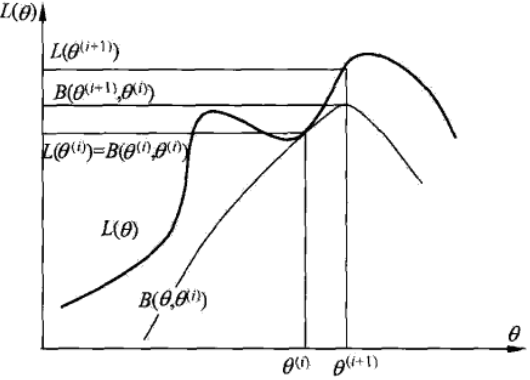
\includegraphics[scale=.50]{EM-algorithm.png}
\caption{Graphical interpretation of a single iteration of the EM algorithm: The function $B(\vec{\theta},\vec{\theta}^{(i)})$ is bounded above by the log likelihood function $\ell(\vec{\theta})$. The functions are equal at $\vec{\theta} = \vec{\theta}^{(i)}$. The EM algorithm chooses $\vec{\theta}^{(i)}$ as the value of $\vec{\theta}$ for which $B(\vec{\theta},\vec{\theta}^{(i)})$ is a maximum. Since $\ell(\vec{\theta}) \geq B(\vec{\theta},\vec{\theta}^{(i)})$ increasing $B(\vec{\theta},\vec{\theta}^{(i)})$ ensures that the value of the log likelihood function $\ell(\vec{\theta})$ is increased at each step.}
\label{fig:EM-algorithm} 
\end{figure}


\section{Examples}

\subsection{Gaussian mixture model}
\begin{definition}
In Gaussian mixture model(GMM) model, each base distribution in the mixture is a multivariate Gaussian with mean $\mu_k$ and covariance matrix $\sigma_k$. Thus the model has the form
\begin{equation}
P(x_i|\vec{\theta})=\sum\limits_{k=1}^K{\pi_k\phi(x_i|\mu_k,\sigma_k)}
\end{equation}
\end{definition}

Figure ~\ref{fig:GMM} shows a mixture of 3 Gaussians in 2D. Each mixture component is represented by a different set of eliptical contours. Given a sufficiently large number of mixture components, a GMM can be used to approximate any density defined on $\mathbb{R}^D$.

\begin{figure}[hbtp]
\centering
    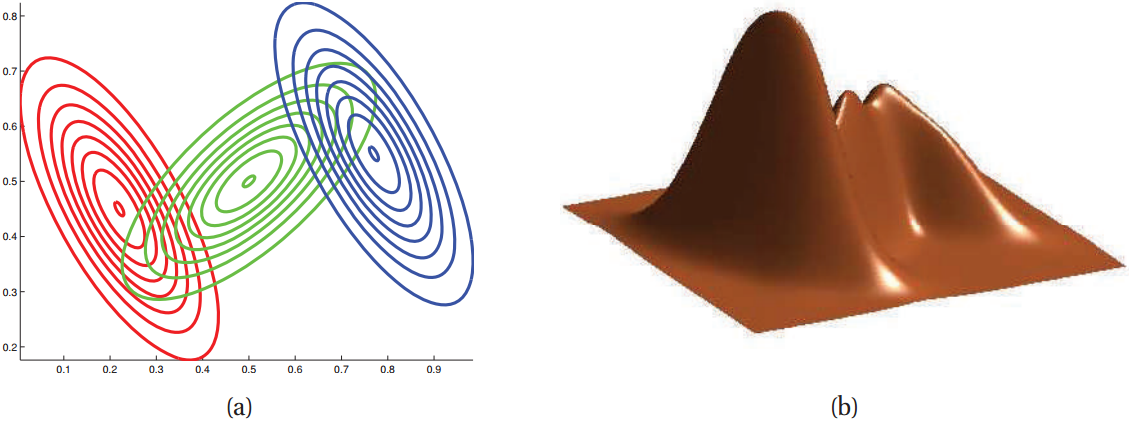
\includegraphics[scale=.50]{GMM.png}
\caption{A mixture of 3 Gaussians in 2d. (a) We show the contours of constant probability for eachcomponent in the mixture. (b) A surface plot of the overall density.}
\label{fig:GMM} 
\end{figure}


\subsubsection{Identify hidden variable, write out the log likelihood function}
Denote the hidden variable as $\gamma_{jk}$, which's meanining is:
\begin{equation}\nonumber
\gamma_{jk}=\begin{cases}
1, & \text{the j-th sample comes from the k-th model}\\
0, & \text{otherwise} \\
\end{cases}
\end{equation}

Given observed sample $x_j$ and hidden variable $\gamma_{jk}$, the complete sample is $(x_j,\gamma_{j1},\gamma_{j1},\cdots,\gamma_{jk})$.

Then the log likelihood function can be written as follows:
\begin{eqnarray}
P(\mathcal{X},\gamma|\vec{\theta}) &=& \prod\limits_{j=1}^N P(x_j,\gamma_{j1},\gamma_{j1},\cdots,\gamma_{jk}|\vec{\theta})\nonumber \\
       &=& \prod\limits_{j=1}^N\left\{\prod\limits_{k=1}^K\left[\pi_k\phi(x_i|\mu_k,\sigma_k)\right]^{\gamma_{jk}}\right\} \nonumber \\
	   &=& \prod\limits_{k=1}^K\left\{\prod\limits_{j=1}^N\left[\pi_k\phi(x_i|\mu_k,\sigma_k)\right]^{\gamma_{jk}}\right\} \nonumber \\
	   &=& \prod\limits_{k=1}^K\left\{\pi_k^{n_k}\prod\limits_{j=1}^N\left[\phi(x_i|\mu_k,\sigma_k)\right]^{\gamma_{jk}}\right\} \nonumber \\
	   &=& \prod\limits_{k=1}^K\left\{\pi_k^{n_k}\prod\limits_{j=1}^N\left[\dfrac{1}{\sqrt{2\pi}\Sigma_k}\exp{\left(-\dfrac{\left(x_j-\mu_k\right)^2}{2\sigma_k^2}\right)}\right]^{\gamma_{jk}}\right\} \nonumber \\
	   && \text{where } n_k=\sum\limits_{j=1}^N{\gamma_{jk}}, \sum\limits_{k=1}^K{n_k}=N. \nonumber \\
\Rightarrow \nonumber \\
\log{P(\mathcal{X},\gamma|\vec{\theta})} &=& \sum\limits_{k=1}^K\left\{n_k\log\pi_k+\sum\limits_{j=1}^N{\gamma_{jk}\left[\log(\dfrac{1}{\sqrt{2\pi}}-\log\sigma_k-\dfrac{\left(x_j-\mu_k\right)^2}{2\sigma_k^2})\right]}\right\}
\end{eqnarray}


\subsubsection{E-step: derive the formula of $Q(\vec{\theta}, \vec{\theta}^{(i)})$}
\begin{eqnarray}
Q(\vec{\theta}, \vec{\theta}^{(i)}) &=& \mathbb{E}_{\vec{z}|\mathcal{X},\theta^{(i)}}\log\left[P(\mathcal{X},\vec{z}|\vec{\theta})\right] \nonumber \\
    &=& \mathbb{E}_{\vec{\gamma}|\mathcal{X},\theta^{(i)}}\left\{\sum\limits_{k=1}^K\left\{n_k\log\pi_k+\sum\limits_{j=1}^N{\gamma_{jk}\left[\log(\dfrac{1}{\sqrt{2\pi}}-\log\sigma_k-\dfrac{\left(x_j-\mu_k\right)^2}{2\sigma_k^2})\right]}\right\}\right\} \nonumber \\
	&=& \sum\limits_{k=1}^K\left\{\left(\sum\limits_{j=1}^N{E\gamma_{jk}}\right)\log\pi_k+\sum\limits_{j=1}^N{E\gamma_{jk}\left[\log(\dfrac{1}{\sqrt{2\pi}}-\log\sigma_k-\dfrac{\left(x_j-\mu_k\right)^2}{2\sigma_k^2})\right]}\right\} \nonumber \\
	&& \text{denote } E\gamma_{jk} \text{ as } \hat{\gamma}_{jk} \nonumber \\
	&=& \sum\limits_{k=1}^K\left\{\left(\sum\limits_{j=1}^N{\hat{\gamma}_{jk}}\right)\log\pi_k+\sum\limits_{j=1}^N{\hat{\gamma}_{jk}\left[\log(\dfrac{1}{\sqrt{2\pi}}-\log\sigma_k-\dfrac{\left(x_j-\mu_k\right)^2}{2\sigma_k^2})\right]}\right\} \label{eqn:Q-function} \label{eqn:Q-function}
\end{eqnarray}

\begin{eqnarray}
\hat{\gamma}_{jk} &=& E\gamma_{jk} = E(\gamma_{jk}|x_j,\vec{\theta})=E(\gamma_{jk}=1|x_j,\vec{\theta}) \nonumber \\
	&=& \dfrac{P(\gamma_{jk}=1, x_j|\vec{\theta})}{\sum\limits_{k=1}^K{P(\gamma_{jk}=1, x_j|\vec{\theta})}} \nonumber \\
	&=& \dfrac{P(x_j|\gamma_{jk}=1, \vec{\theta})P(\gamma_{jk}=1, \vec{\theta})}{\sum\limits_{k=1}^K{P(x_j|\gamma_{jk}=1, \vec{\theta})P(\gamma_{jk}=1, \vec{\theta})}} \nonumber \\
	&=& \dfrac{\phi(x_i|\mu_k,\sigma_k)\pi_k}{\sum\limits_{k=1}^K{\phi(x_i|\mu_k,\sigma_k)\pi_k}} \nonumber \\
	&=& \dfrac{\pi_k\phi(x_i|\mu_k,\sigma_k)}{\sum\limits_{k=1}^K{\pi_k\phi(x_i|\mu_k,\sigma_k)}} \nonumber
\end{eqnarray}
Use this formula to update $\hat{\gamma}_{jk}$.

\subsubsection{M-step: find \vec{\theta} that maximizes the value of $Q(\vec{\theta}, \vec{\theta}^{(i)})$}
Take partial derivatives of Eqn.\eqref{eqn:Q-function} with respect to $\mu_k$, $\sigma_k^2$ and let them equal to 0, we can get $\mu_k$, $\sigma_k^2$.
\begin{eqnarray}
\dfrac{\partial}{\partial \mu_k}Q(\vec{\theta}, \vec{\theta}^{(i)}) &=& \sum\limits_{j=1}^N{\hat{\gamma}_{jk}\left[-\dfrac{1}{2\sigma_k^2} \cdot 2\left(x_j-\mu_k\right) \cdot (-1)\right]} = 0 \nonumber \\
\sum\limits_{j=1}^N{\hat{\gamma}_{jk}\left[\left(x_j-\mu_k\right)\right]} &=& 0 \nonumber \\
\hat{\mu}_k &=& \dfrac{\sum\limits_{j=1}^N{\hat{\gamma}_{jk}x_j}}{\hat{\gamma}_{jk}}
\end{eqnarray}

\begin{eqnarray}
\dfrac{\partial}{\partial \sigma_k^2}Q(\vec{\theta}, \vec{\theta}^{(i)}) &=& \sum\limits_{j=1}^N{\hat{\gamma}_{jk}\left[-\dfrac{1}{2\sigma_k^2}+\dfrac{1}{2\sigma_k^4}\left(x_j-\mu_k\right)^2\right]} = 0 \nonumber \\
\sum\limits_{j=1}^N{\hat{\gamma}_{jk}\left[-\sigma_k^2+\left(x_j-\mu_k\right)^2\right]} &=& 0 \nonumber \\
\hat{\sigma}_k^2 &=& \dfrac{\sum\limits_{j=1}^N{\hat{\gamma}_{jk}\left(x_j-\mu_k\right)^2}}{\hat{\gamma}_{jk}}
\end{eqnarray}

Grouping together only the terms that depend on $\pi_k$, we find that we need to maximize $\sum\limits_{k=1}^K{\left(\sum\limits_{j=1}^N{\hat{\gamma}_{jk}}\right)\log\pi_k}$. However, there is an additional constraint $\sum\limits_{k=1}^K{\pi_k}=1$, since they represent the probabilities $\vec{\pi}_k=P(x^{(i)}=k|\vec{\pi})$. To deal with the constraint we construct the Lagrangian
\begin{equation}
\mathcal{L}(\vec{\pi})=\sum\limits_{k=1}^K{\left(\sum\limits_{j=1}^N{\hat{\gamma}_{jk}}\right)\log\pi_k}+\beta\left(\sum\limits_{k=1}^K{\pi_k}-1\right) \nonumber
\end{equation}

where $\beta$ is the Lagrange multiplier. Taking derivatives, we find
\begin{equation}
\hat{\vec{\pi}}_k=\dfrac{\sum\limits_{k=1}^K{\hat{\gamma}_{jk}}}{N}
\end{equation}


\subsubsection{EM algorithm for GMM}

\begin{algorithm}[htbp]
    \SetAlgoNoLine
    \SetKwInOut{Input}{input}\SetKwInOut{Output}{output}
    \Input{observed data $\mathcal{X}=\{\vec{x}^{(1)},\vec{x}^{(2)},\cdots, \vec{x}^{(n)}$\},GMM}
	\Output{GMM's parameters $\vec{\pi},\vec{\mu},\vec{\sigma}$}

	// 1. initialize \\
	$\vec{\pi}^{(0)}$ = ... \\
	$\vec{\mu}^{(0)}$ = ...  \\
	$\vec{\sigma}^{(0)}$ = ...  \\
	
	\While{(!convergency)} {
	    // 2. E-step \\
	    $\hat{\gamma}_{jk}=\dfrac{\pi_k\phi(x_i|\mu_k,\sigma_k)}{\sum\limits_{k=1}^K{\pi_k\phi(x_i|\mu_k,\sigma_k)}}$ \\
	    // 3. M-step \\
		$\hat{\mu}_k = \dfrac{\sum\limits_{j=1}^N{\hat{\gamma}_{jk}x_j}}{\hat{\gamma}_{jk}}$ \\
		$\hat{\sigma}_k^2 = \dfrac{\sum\limits_{j=1}^N{\hat{\gamma}_{jk}\left(x_j-\mu_k\right)^2}}{\hat{\gamma}_{jk}}$ \\
		$\hat{\vec{\pi}}_k=\dfrac{\sum\limits_{k=1}^K{\hat{\gamma}_{jk}}}{N}$ \\
	}
	
\caption{EM algorithm for GMM}
\end{algorithm}


\section{Generalization of EM Algorithm}
EM algorithm can be interpreted as F function's maximization-maximization algorithm, based on this interpretation there are many variations and generalization, e.g., generalized EM Algorithm(GEM).


\subsection{F function's maximization-maximization algorithm}
\begin{definition}
Given the probability distribution of the hidden variable $Z$ is $\tilde{P}(Z)$, define \textbf{F function} as the following:
\begin{equation}
F(\tilde{P},\vec{\theta})=\mathbb{E}_{\tilde{P}}\left[\log{P(X,Z|\theta)}\right]+H(\tilde{P})
\end{equation}
Where $H(\tilde{P})=-\mathbb{E}_{\tilde{P}}\log\tilde{P}(Z)$, which is $\tilde{P}(Z)$'s entropy. Usually we assume that $P(X,Z|\theta)$ is continuous w.r.t. $\vec{\theta}$, therefore $F(\tilde{P},\vec{\theta})$ is continuous w.r.t. $\tilde{P}$ and $\vec{\theta}$.
\end{definition}

\begin{lemma}
\label{lemma:F-function}
For a fixed $\vec{\theta}$, there is only one distribution $\tilde{P}_{\theta}$ which maximizes $F(\tilde{P},\vec{\theta})$
\begin{equation}
\tilde{P}_{\theta}(Z)=P(Z|X, \vec{\theta})
\end{equation}
and $\tilde{P}_{\theta}$ is continuous w.r.t. $\vec{\theta}$.
\end{lemma}

\begin{proof}
Given a fixed $\vec{\theta}$, we can get $\tilde{P}_{\theta}$ which maximizes $F(\tilde{P},\vec{\theta})$. we construct the Lagrangian
\begin{equation}
\mathcal{L}(\tilde{P}, \vec{\theta})=\mathbb{E}_{\tilde{P}}\left[\log{P(X,Z|\theta)}\right]-\mathbb{E}_{\tilde{P}}\log\tilde{P}_{\theta}(Z)+\lambda\left[1-\sum\limits_Z{\tilde{P}(Z)}\right]
\end{equation}

Take partial derivative with respect to $\tilde{P}_{\theta}(Z)$ then we get
\begin{equation}
\dfrac{\partial \mathcal{L}}{\partial{\tilde{P}_{\theta}(Z)}}=\log{P(X,Z|\theta)}-\log\tilde{P}_{\theta}(Z)-1-\lambda  \nonumber
\end{equation}

Let it equal to 0, we can get
\begin{equation}
\lambda=\log{P(X,Z|\theta)}-\log\tilde{P}_{\theta}(Z)-1 \nonumber
\end{equation}

Then we can derive that $\tilde{P}_{\theta}(Z)$ is proportional to $P(X,Z|\theta)$
\begin{eqnarray}
\dfrac{P(X,Z|\theta)}{\tilde{P}_{\theta}(Z)} &=& e^{1+\lambda} \nonumber \\
\Rightarrow \tilde{P}_{\theta}(Z) &=& \dfrac{P(X,Z|\vec{\theta})}{e^{1+\lambda}} \nonumber \\
\sum\limits_Z{\tilde{P}_{\theta}(Z)}=1 & \Rightarrow & \sum\limits_Z{\dfrac{P(X,Z|\vec{\theta})}{e^{1+\lambda}}}=1 \Rightarrow P(X|\vec{\theta})=e^{1+\lambda} \nonumber \\
\tilde{P}_{\theta}(Z) &=& \dfrac{P(X,Z|\vec{\theta})}{e^{1+\lambda}} = \dfrac{P(X,Z|\vec{\theta})}{P(X|\vec{\theta})}=P(Z|X, \vec{\theta}) \nonumber
\end{eqnarray}
\end{proof}

\begin{lemma}
If $\tilde{P}_{\theta}(Z)=P(Z|X, \vec{\theta})$, then
\begin{equation}
F(\tilde{P},\vec{\theta})=\log P(X|\vec{\theta})
\end{equation}
\end{lemma}

\begin{theorem}
One iteration of EM algorithm can be implemented as F function's maximization-maximization.

Assume $\vec{\theta}^{(i)}$ is the estimation of $\vec{\theta}$ in the i-th iteration, $\tilde{P}^{(i)}$ is the estimation of $\tilde{P}$ in the i-th iteration. Then in the (i+1)-th iteration two steps are:
\begin{enumerate}
\item for fixed $\vec{\theta}^{(i)}$, find $\tilde{P}^{(i+1)}$ that maximizes $F(\tilde{P},\vec{\theta}^{(i)})$;
\item for fixed $\tilde{P}^{(i+1)}$, find $\vec{\theta}^{(i+1)}$ that maximizes $F(\tilde{P}^{(i+1)},\vec{\theta})$.
\end{enumerate}
\end{theorem}

\begin{proof}
(1) According to Lemma \ref{lemma:F-function}, we can get
\begin{equation}
\tilde{P}^{(i+1)}(Z)=P(Z|X, \vec{\theta}^{(i)}) \nonumber
\end{equation}

(2) According above, we can get
\begin{eqnarray}
F(\tilde{P}^{(i+1)},\vec{\theta}) &=& \mathbb{E}_{\tilde{P}^{(i+1)}}\left[\log{P(X,Z|\theta)}\right]+H(\tilde{P}^{(i+1)}) \nonumber \\
    &=& \sum\limits_Z{P(Z|X,\vec{\theta}^{(i)})\log{P(X,Z|\theta)}}+H(\tilde{P}^{(i+1)}) \nonumber \\
	&=& Q(\vec{\theta}, \vec{\theta}^{(i)})+H(\tilde{P}^{(i+1)})\nonumber
\end{eqnarray}

Then
\begin{equation}
\vec{\theta}^{(i+1)}=\arg\max\limits_{\theta}F(\tilde{P}^{(i+1)},\vec{\theta})=\arg\max\limits_{\theta}Q(\vec{\theta}, \vec{\theta}^{(i)}) \nonumber
\end{equation}
\end{proof}


\subsection{The Generalized EM Algorithm(GEM)}
In the formulation of the EM algorithm described above, $\vec{\theta}^{(i+1)}$ was chosen as the value of $\vec{\theta}$ for which $Q(\vec{\theta}, \vec{\theta}^{(i)})$ was maximized. While this ensures the greatest increase in $\ell(\vec{\theta})$, it is however possible to relax the requirement of maximization to one of simply increasing $Q(\vec{\theta}, \vec{\theta}^{(i)})$ so that $Q(\vec{\theta}^{(i+1)}, \vec{\theta}^{(i)}) \geq Q(\vec{\theta}^{(i)}, \vec{\theta}^{(i)})$. This approach, to simply increase and not necessarily maximize $Q(\vec{\theta}^{(i+1)}, \vec{\theta}^{(i)})$ is known as the Generalized Expectation Maximization (GEM) algorithm and is often useful in cases where the maximization is difficult. The convergence of the GEM algorithm is similar to the EM algorithm.


\section{Reference}
[1] Dempster AP, Laird NM, Rubin DB. Maximum-likelihood from incomplete data via the EM algorithm. J.Royal Statist. Soc. Ser.B., 1977, 39

[2] Sean Borman. The Expectation Maximization Algorithm A short tutorial. 2009. \url{http://www.seanborman.com/publications/EM_algorithm.pdf}
\chapter{Hidden markov Model}


\section{Introduction}


\section{Markov models}
\label{sec:Markov-models}


\chapter{BayesNets}
\section{Chain rule}
\begin{equation}
p(x) = p(x_1)\prod_{v = 2}^Vp(x_v|x_{1:v-1})
\end{equation}

\section{Markov chain}
\begin{equation}
p(x) = p(x_1)\prod_{v = 2}^Vp(x_v|x_{v-1})
\end{equation}

\section{DGM}
\begin{equation}
p(x|G) = \prod_{v=1}^Vp(x_v|x_{pa(v)})
\label{bayes_net}
\end{equation}

\section{Inference}
\begin{equation}
p(x_h|x_v,\theta) = 
\frac{p(x_h, x_v|\theta)}
{\sum_{x_h'}p(x_h', x_v|\theta)}
\end{equation}

\begin{equation}
p(x_q|x_v,\theta) = \sum_{x_n}p(x_q, x_n|x_v, \theta)
\end{equation}

\section{Learning}
\subsection{MAP}
\begin{equation}
\hat{\theta} =
\underset{\theta}{\operatorname{argmax}}
p(\theta)\prod_{n=1}^Np(x_n|\theta)
\end{equation}
\subsection{Learning from complete data}
\begin{equation}
p(D|\theta) = \prod_{n=1}^Np(x_n|\theta)
= \prod_{n=1}^N\prod_{v=1}^Vp(x_{nv}|x_{n, pa(v)}, \theta_v)
= \prod_{v=1}^Vp(D_v|\theta_v)
\end{equation}

\subsection{Multinoulli Learning}
Multinoulli Distribution:
\begin{equation}
Cat(x|\mu) = \prod_{k=1}^K\mu_k^{x_k}
\label{discrite}
\end{equation}
then from \ref{bayes_net} and \ref{discrite}:
\begin{equation}
p(x|G,\theta) = \prod_{v=1}^V\prod_{c=1}^{C_v}\prod_{k=1}^K
\theta_{vck}^{y_{vck}}
\end{equation}
Likelihood
\begin{equation}
p(D|G,\theta) = \prod_{n=1}^N p(x_n|G,\theta)
=\prod_{n=1}^N\prod_{v=1}^V\prod_{c=1}^{C_{nv}}\prod_{k=1}^K
\theta_{vck}^{y_{nvck}}
\end{equation}
where $y_{nv} = f(pa(x_{nv}))$, f(x) is a map from x to a vector,
there is only one element in the vector is 1.

\section{d-separation}
\begin{enumerate}
\item P contains a chain
\begin{equation}
p(x,z|y) = \frac{p(x,y,z)}{p(y)}
= \frac{p(x)p(y|x)p(z|y)}{p(y)}
= \frac{p(x,y)p(z|y)}{p(y)} = p(x|y)p(z|y)
\end{equation}

\item P contains a fork
\begin{equation}
p(x,z|y) = \frac{p(x,y,z)}{p(y)}
= \frac{p(y)p(x|y)p(z|y)}{p(y)}
= p(x|y)p(z|y)
\end{equation}
\item P contains v-structure
\begin{equation}
p(x,z|y) = \frac{p(x,y,z)}{p(y)}
= \frac{p(x)p(z)p(y|x,z)}{p(y)}
\neq p(x|y)p(z|y)
\end{equation}
\end{enumerate}
\section{Markov blanket}
\begin{equation}
mb(t) = ch(t)\cup pa(t)\cup copa(t)
\end{equation}

\section{Reference}
Mlapp chapter 10 Bayes nets

\chapter{Conditional Random Field}

%

\backmatter%%%%%%%%%%%%%%%%%%%%%%%%%%%%%%%%%%%%%%%%%%%%%%%%%%%%%%%
\appendix
\chapter{Optimization methods}
\label{chap:Optimization-methods}


\section{Gradient descent}
\label{sec:Gradient-descent}


\subsection{Stochastic gradient descent}

\begin{algorithm}[htbp]
    \SetAlgoNoLine
	\SetKwInOut{Input}{input}\SetKwInOut{Output}{output}
	
    \Input{Training data $\mathcal{D}=\left\{(\vec{x}_i,y_i) | i=1:N\right\}$}
	\Output{A linear model: $y_i=\vec{\theta}^T\vec{x}$}
    $\vec{w} \leftarrow 0;\; b \leftarrow 0;\; k \leftarrow 0$\;
    \While{no mistakes made within the for loop}{
        \For{$i\leftarrow 1$ \KwTo $N$}{
			\If{$y_i(\vec{w} \cdot \vec{x}_i+b) \leq 0$}{
				$\vec{w} \leftarrow \vec{w}+\eta y_i \vec{x}_i$\;
				$b \leftarrow b+\eta y_i$\;
				$k \leftarrow k+1$\;
			}
		}
    }
\caption{Stochastic gradient descent}
\end{algorithm}


\subsection{Batch gradient descent}


\section{Lagrange duality}


\subsection{Primal form}
Consider the following, which we'll call the \textbf{primal} optimization problem:
\begin{eqnarray}
xyz
\end{eqnarray}


\subsection{Dual form}


%%%%%%%%%%%%%%%%%%%%%%acronym.tex%%%%%%%%%%%%%%%%%%%%%%%%%%%%%%%%%%%%%%%%%
% sample list of acronyms
%
% Use this file as a template for your own input.
%
%%%%%%%%%%%%%%%%%%%%%%%% Springer %%%%%%%%%%%%%%%%%%%%%%%%%%

\Extrachap{Glossary}

\runinhead{feture vector} A feture vector to represent one data.

\runinhead{loss function} a function that maps an event onto a real number intuitively representing some "cost" associated with the event.

\runinhead{glossary term} Write here the description of the glossary term. Write here the description of the glossary term. Write here the description of the glossary term.

\printindex

%%%%%%%%%%%%%%%%%%%%%%%%%%%%%%%%%%%%%%%%%%%%%%%%%%%%%%%%%%%%%%%%%%%%%%

\end{document}

